\begin{figure}[H]
\centering
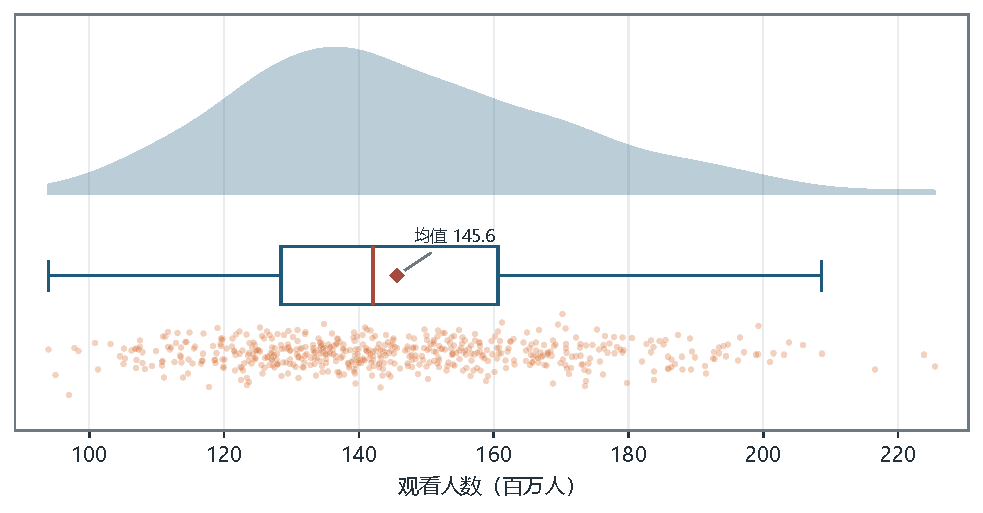
\includegraphics[width=0.82\textwidth]{figures/fig_q1_target_raincloud.pdf}
\caption{训练集观看人数分布与长尾特征}
\label{fig:q1-target-raincloud}
\end{figure}

\begin{figure}[H]
\centering
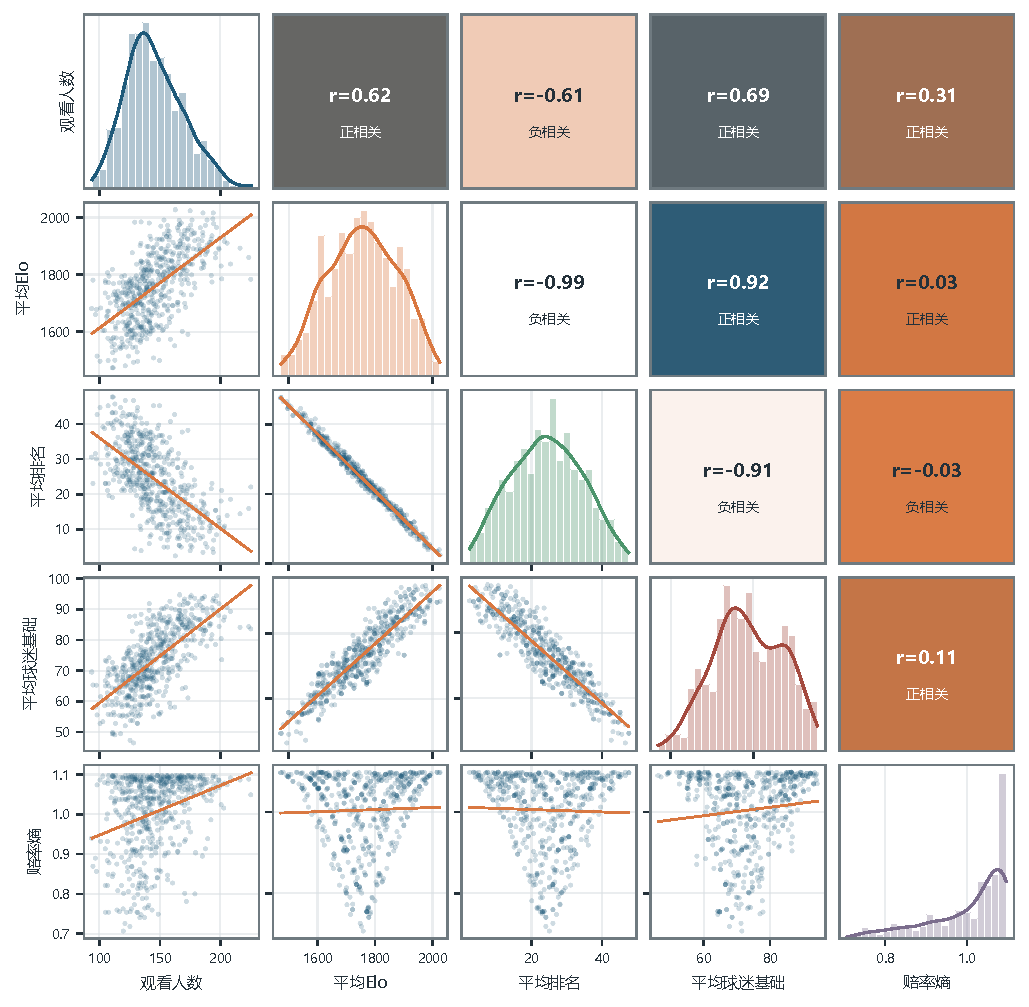
\includegraphics[width=0.88\textwidth]{figures/fig_q1_feature_pairplot.pdf}
\caption{问题一核心赛前特征成对关系}
\label{fig:q1-feature-pairplot}
\end{figure}

\begin{figure}[H]
\centering
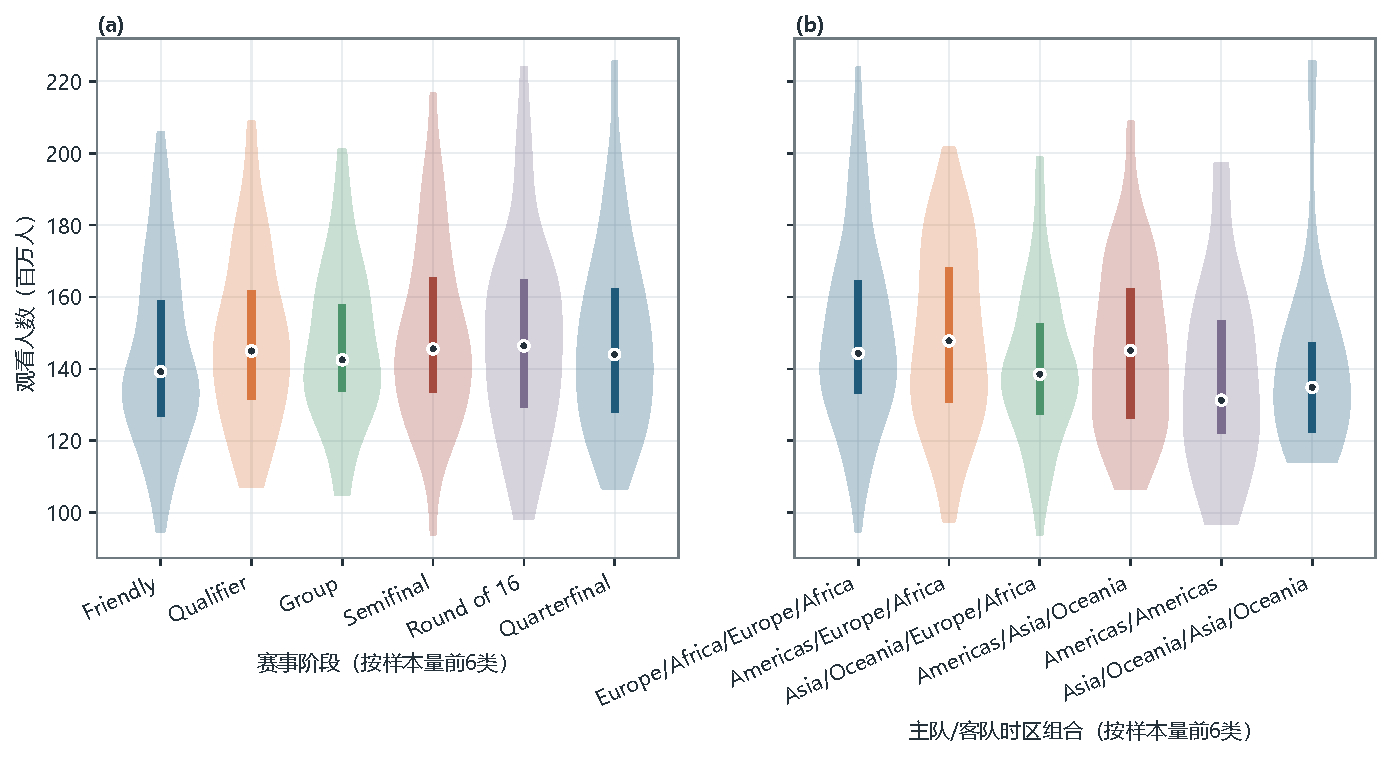
\includegraphics[width=0.96\textwidth]{figures/fig_q1_stage_timezone_violin.pdf}
\caption{赛事阶段与时区组合下观看人数异质性}
\label{fig:q1-stage-timezone-violin}
\end{figure}

\begin{figure}[H]
\centering
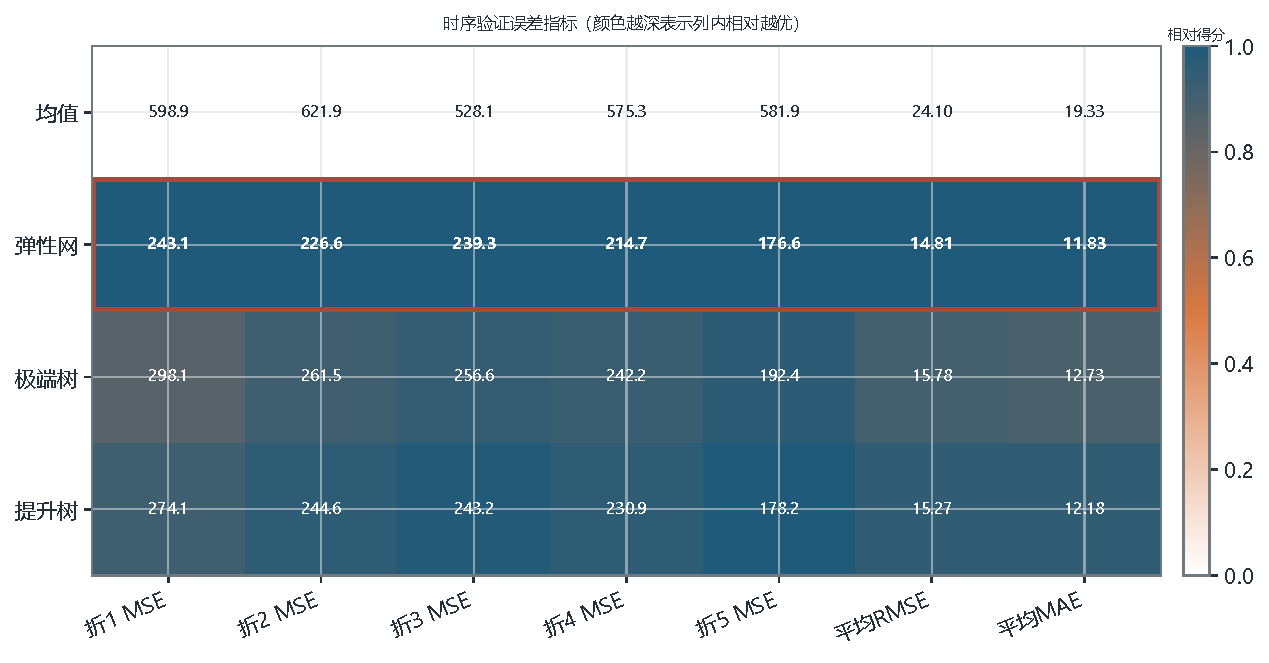
\includegraphics[width=0.90\textwidth]{figures/fig_q1_model_accuracy_heatmap.pdf}
\caption{候选模型时序验证误差比较}
\label{fig:q1-model-accuracy-heatmap}
\end{figure}

\begin{figure}[H]
\centering
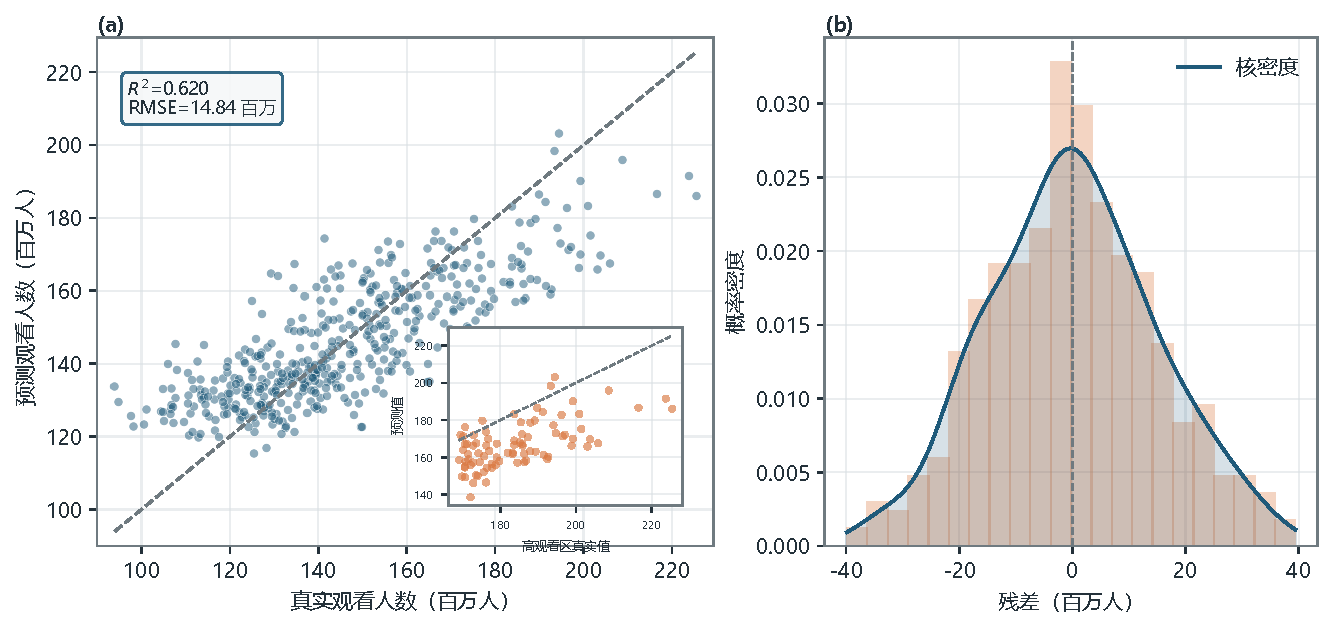
\includegraphics[width=0.94\textwidth]{figures/fig_q1_prediction_fit.pdf}
\caption{最终模型OOF预测拟合与残差分布}
\label{fig:q1-prediction-fit}
\end{figure}

\begin{figure}[H]
\centering
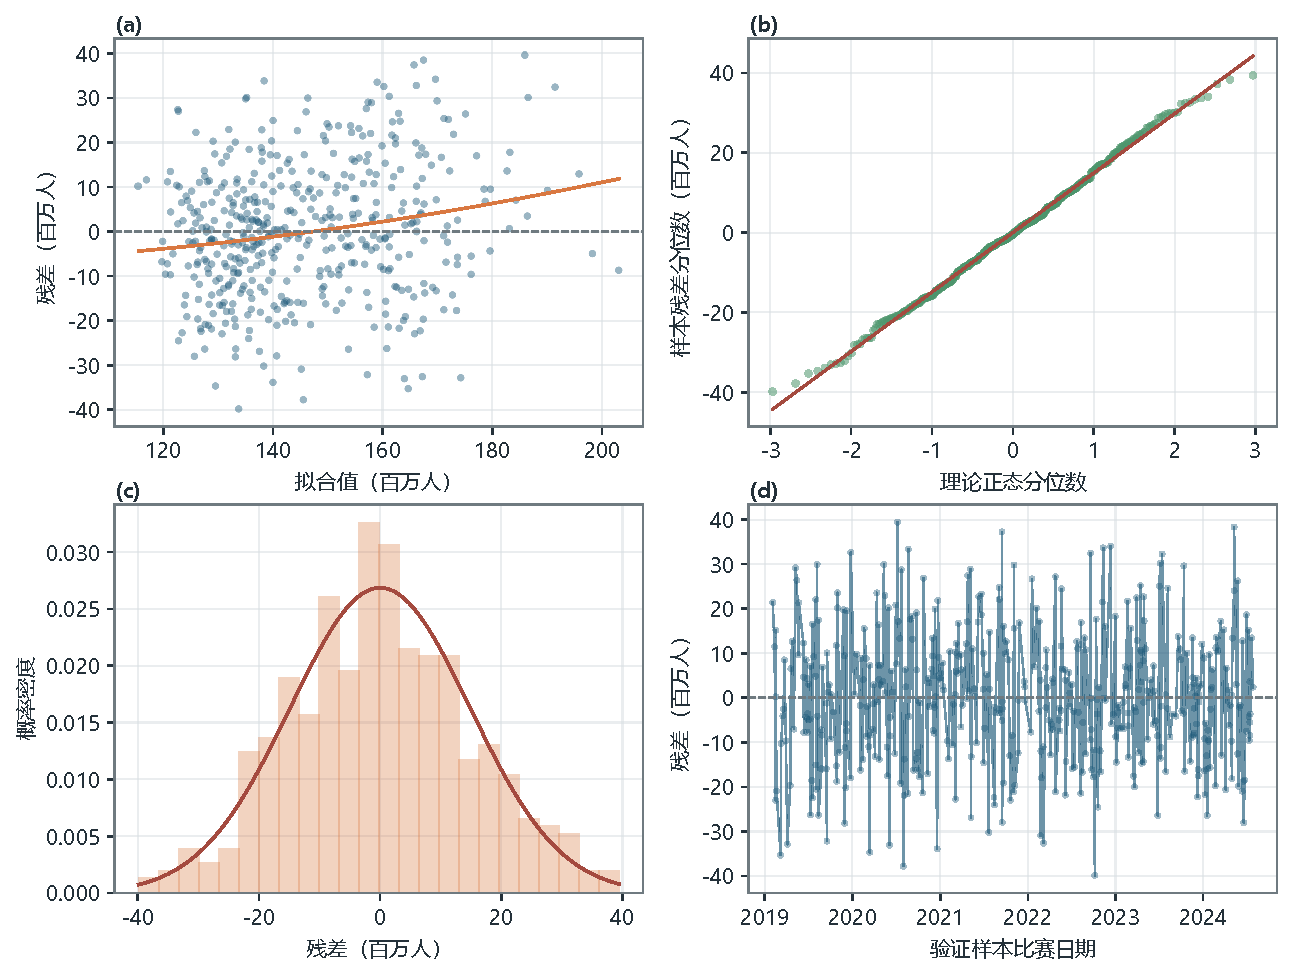
\includegraphics[width=0.92\textwidth]{figures/fig_q1_residual_diagnostics.pdf}
\caption{最终模型残差诊断四联图}
\label{fig:q1-residual-diagnostics}
\end{figure}

\begin{figure}[H]
\centering
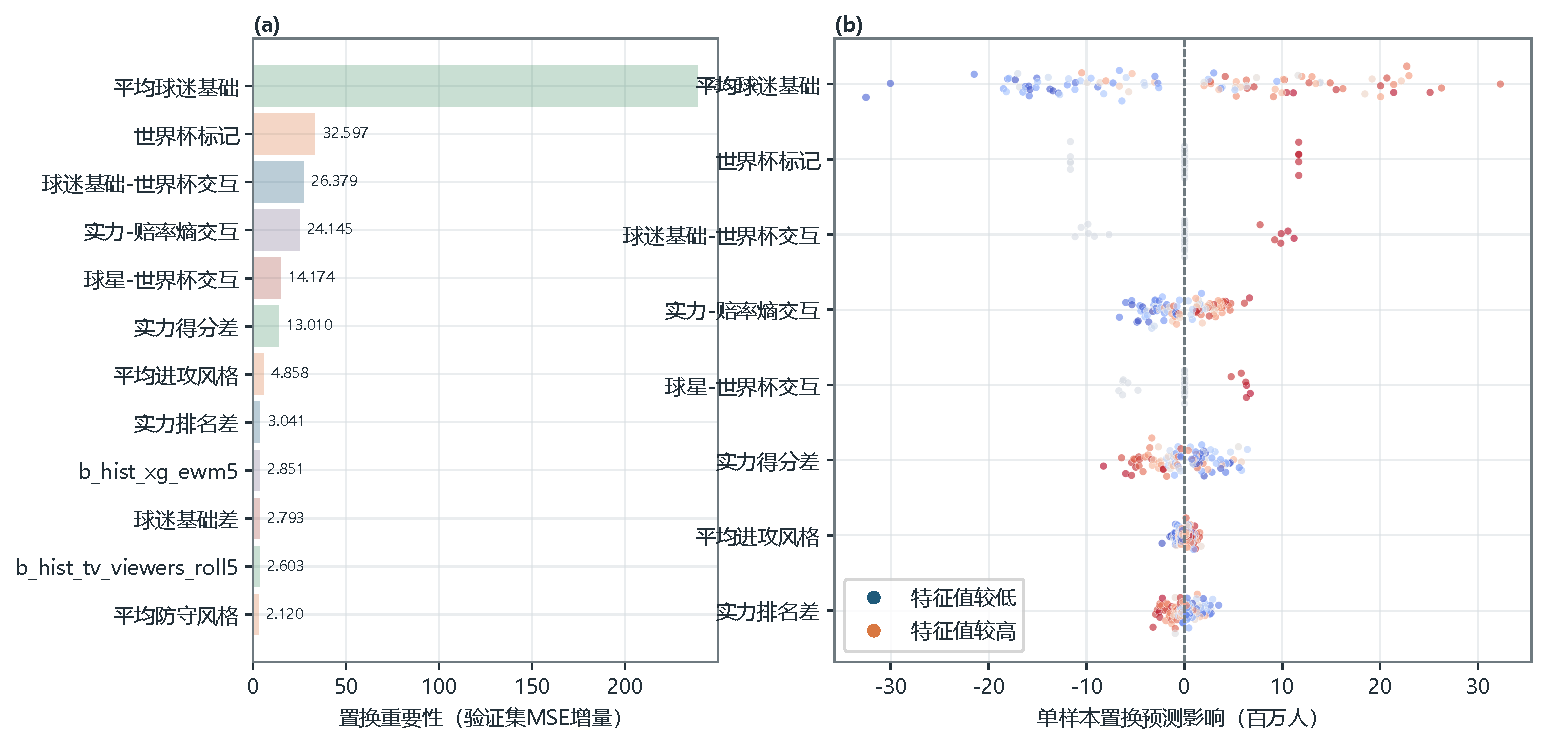
\includegraphics[width=0.96\textwidth]{figures/fig_q1_shap_summary.pdf}
\caption{ElasticNet置换重要性与单样本预测影响}
\label{fig:q1-shap-summary}
\end{figure}

\begin{figure}[H]
\centering
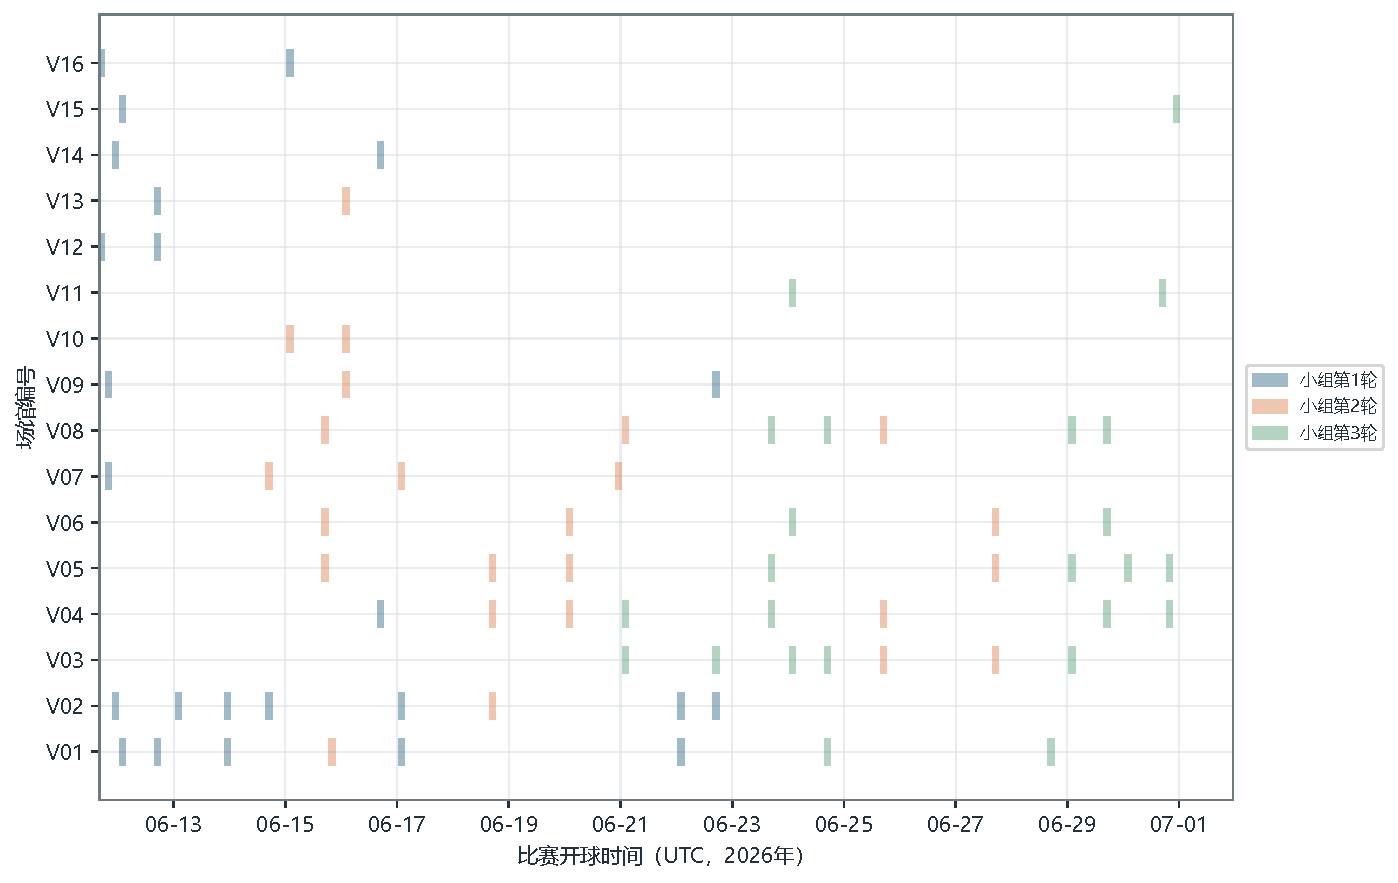
\includegraphics[width=0.98\textwidth]{figures/fig_q2_schedule_gantt.pdf}
\caption{72场小组赛UTC排程甘特图}
\label{fig:q2-schedule-gantt}
\end{figure}

\begin{figure}[H]
\centering
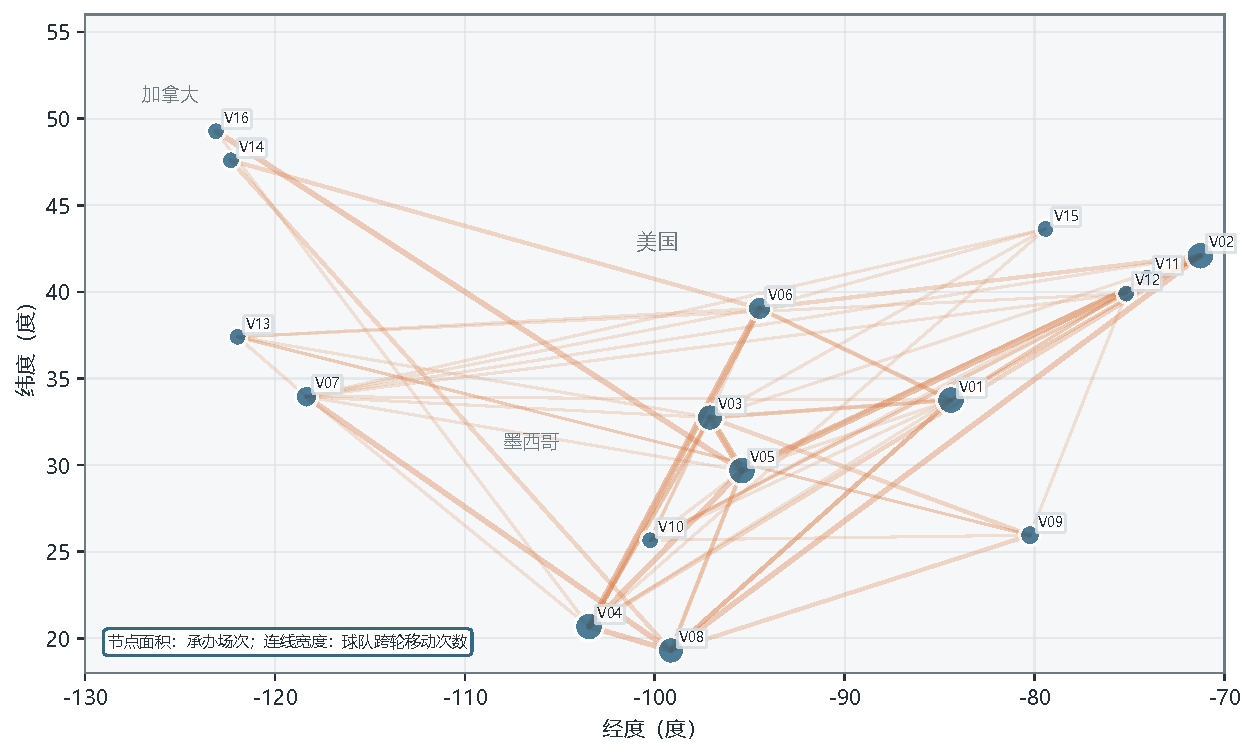
\includegraphics[width=0.92\textwidth]{figures/fig_q2_venue_travel_map.pdf}
\caption{场馆负载与球队跨轮旅行网络}
\label{fig:q2-venue-travel-map}
\end{figure}

\begin{figure}[H]
\centering
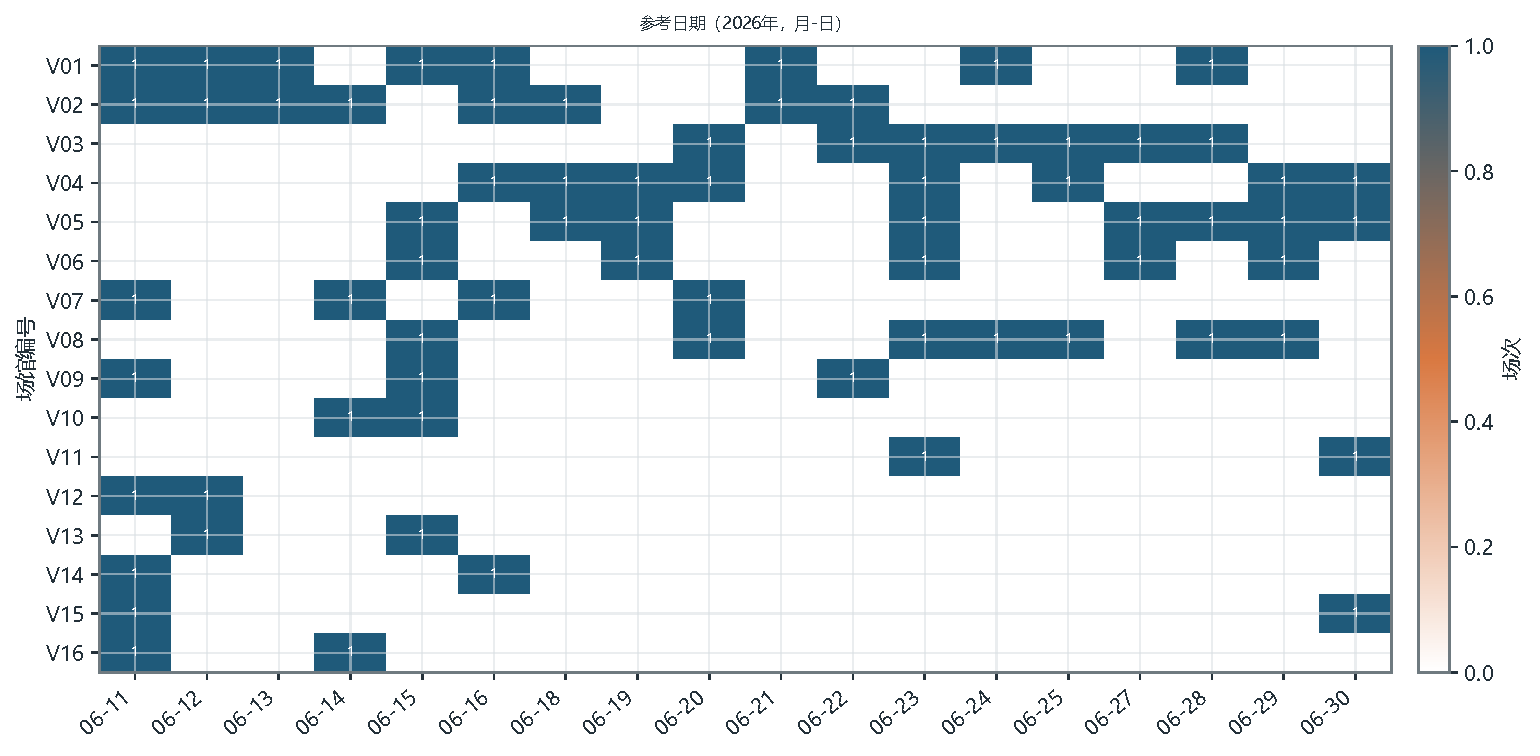
\includegraphics[width=0.98\textwidth]{figures/fig_q2_venue_slot_matrix.pdf}
\caption{场馆与参考日期占用矩阵}
\label{fig:q2-venue-slot-matrix}
\end{figure}

\begin{figure}[H]
\centering
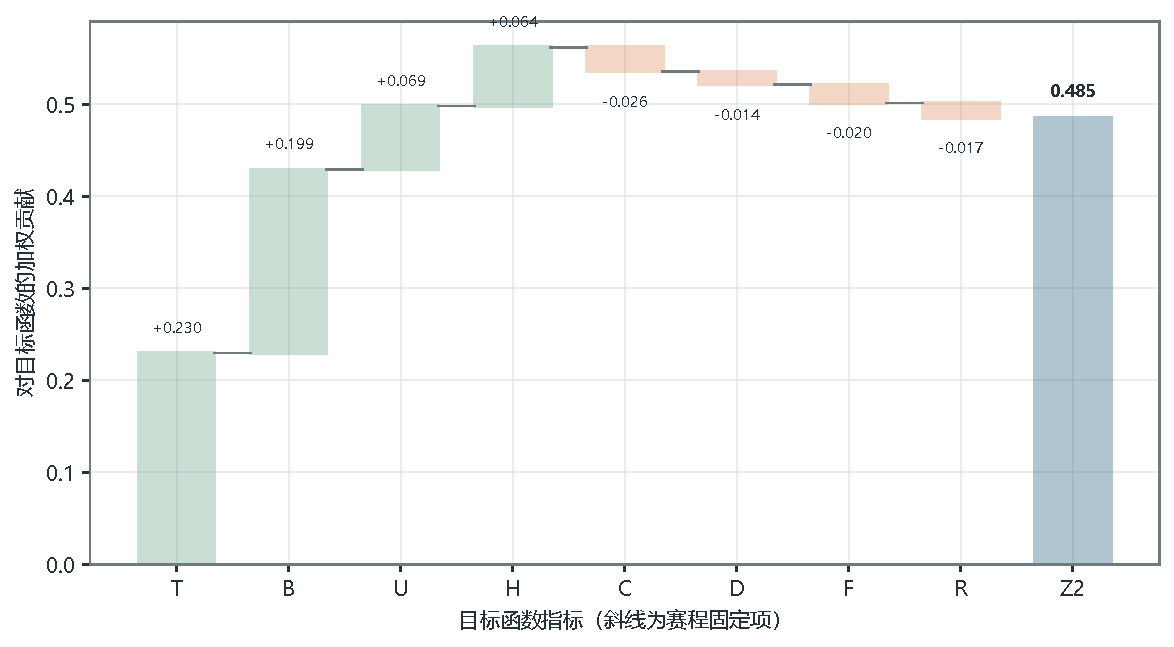
\includegraphics[width=0.90\textwidth]{figures/fig_q2_objective_waterfall.pdf}
\caption{问题二目标函数八项贡献分解}
\label{fig:q2-objective-waterfall}
\end{figure}

\begin{figure}[H]
\centering
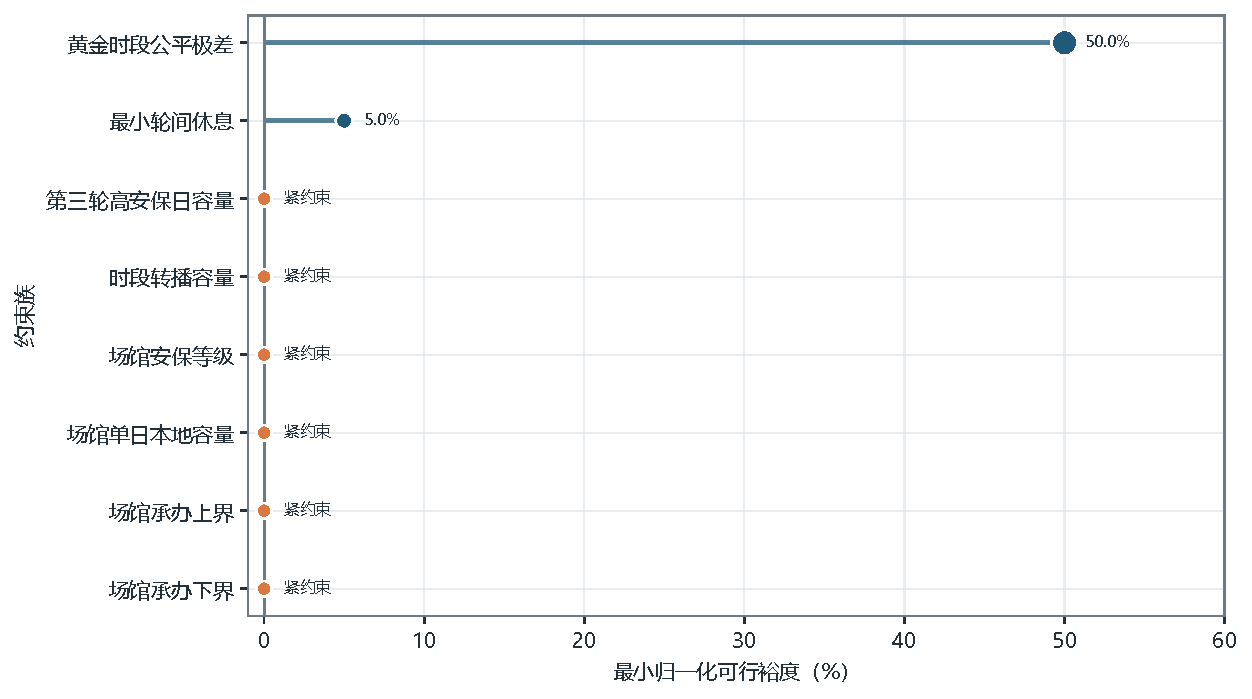
\includegraphics[width=0.86\textwidth]{figures/fig_q2_constraint_margins_lollipop.pdf}
\caption{问题二最紧约束归一化裕度}
\label{fig:q2-constraint-margins-lollipop}
\end{figure}

\begin{figure}[H]
\centering
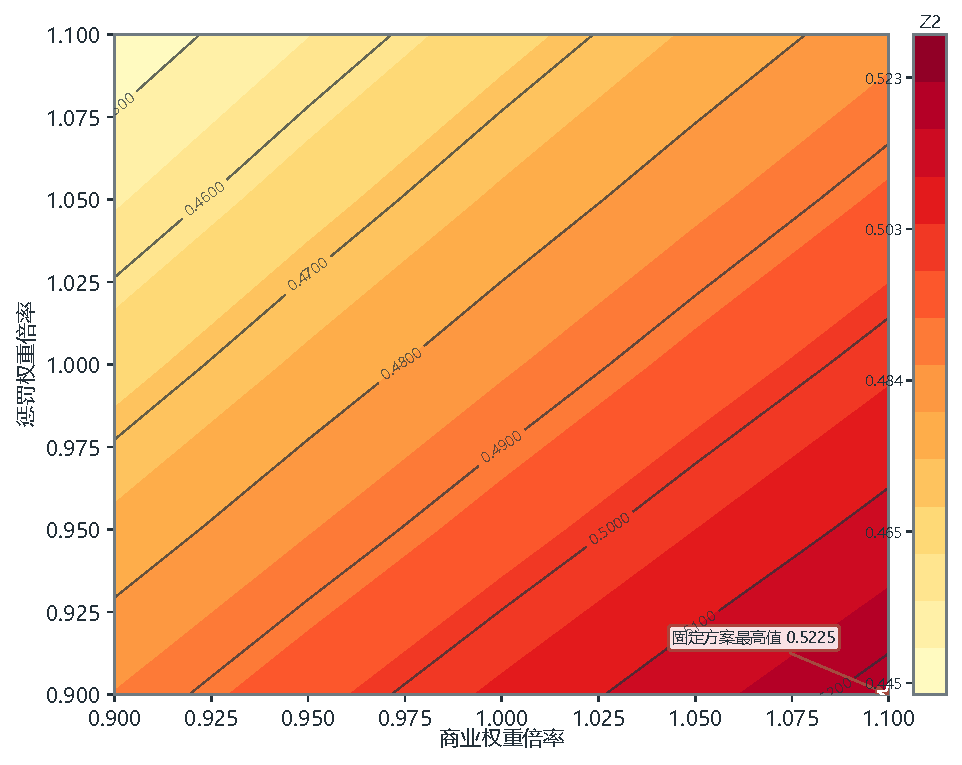
\includegraphics[width=0.78\textwidth]{figures/fig_q2_weight_sensitivity_contour.pdf}
\caption{商业与惩罚权重联合灵敏度}
\label{fig:q2-weight-sensitivity-contour}
\end{figure}

\begin{figure}[H]
\centering
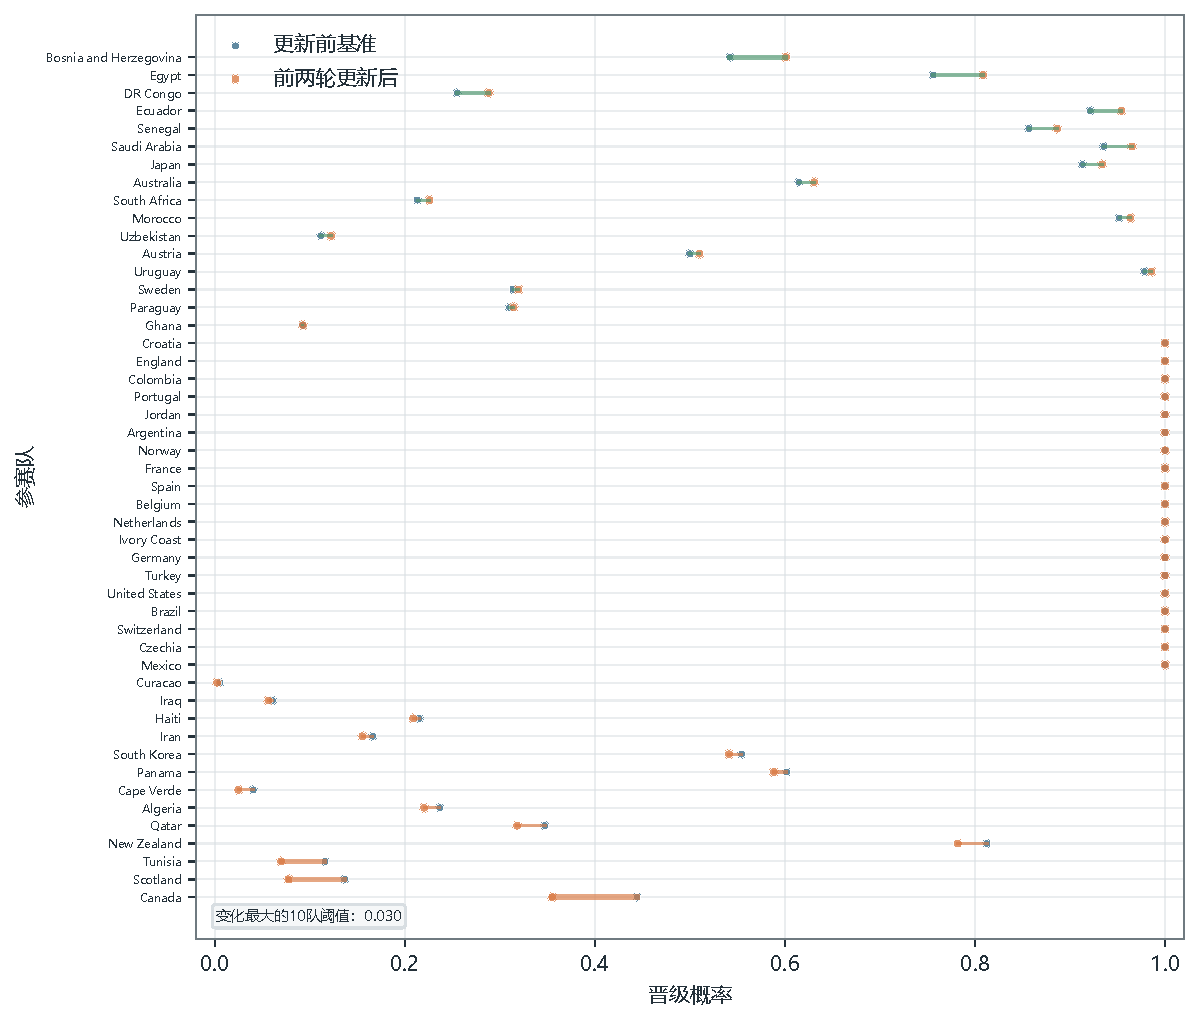
\includegraphics[width=0.82\textwidth]{figures/fig_q3_advancement_shift.pdf}
\caption{更新前后48队晋级概率变化}
\label{fig:q3-advancement-shift}
\end{figure}

\begin{figure}[H]
\centering
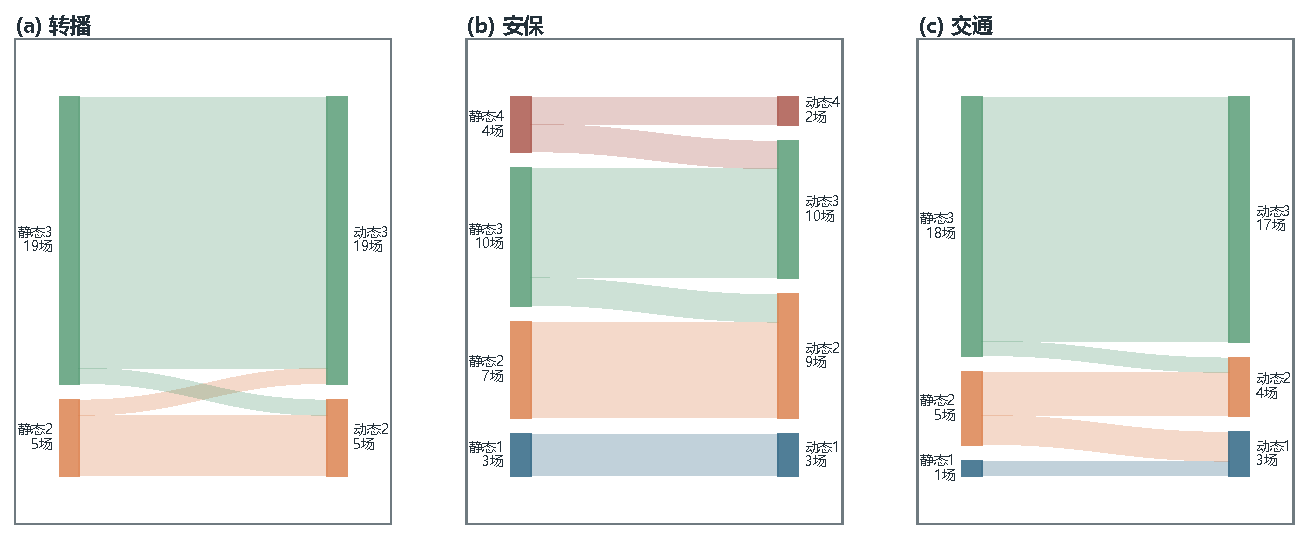
\includegraphics[width=0.96\textwidth]{figures/fig_q3_resource_transition_sankey.pdf}
\caption{静态策略到动态策略的资源等级流转}
\label{fig:q3-resource-transition-sankey}
\end{figure}

\begin{figure}[H]
\centering
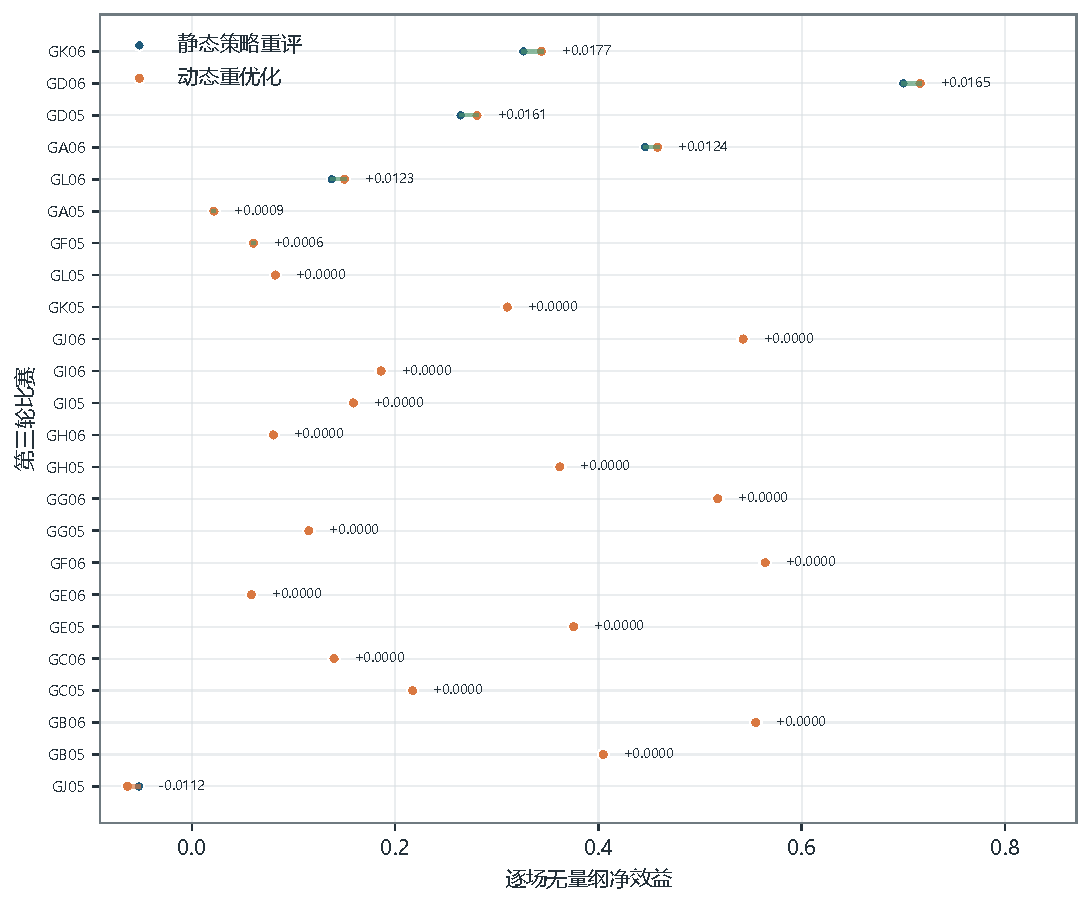
\includegraphics[width=0.86\textwidth]{figures/fig_q3_dynamic_value_dumbbell.pdf}
\caption{24场静态与动态净效益配对比较}
\label{fig:q3-dynamic-value-dumbbell}
\end{figure}

\begin{figure}[H]
\centering
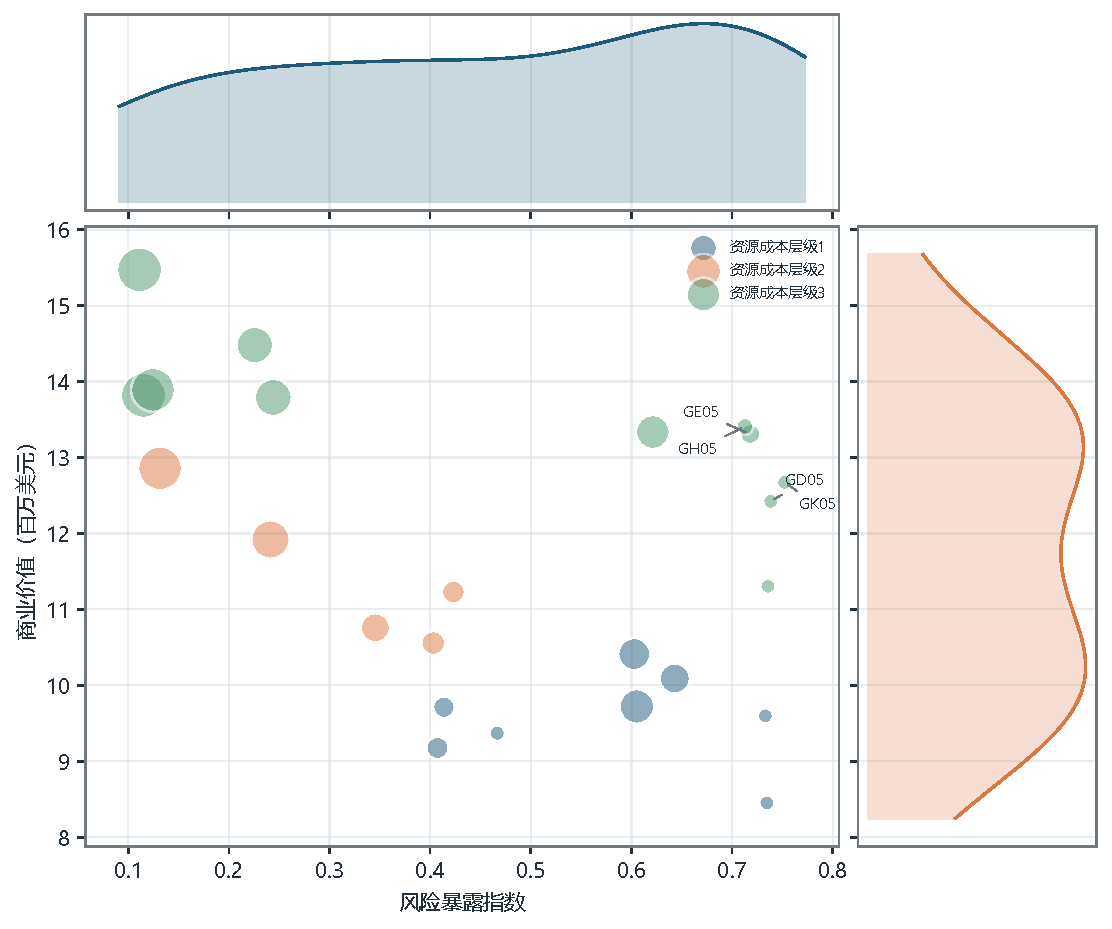
\includegraphics[width=0.82\textwidth]{figures/fig_q3_risk_value_bubble_kde.pdf}
\caption{风险暴露与商业价值联合分布}
\label{fig:q3-risk-value-bubble-kde}
\end{figure}

\begin{figure}[H]
\centering
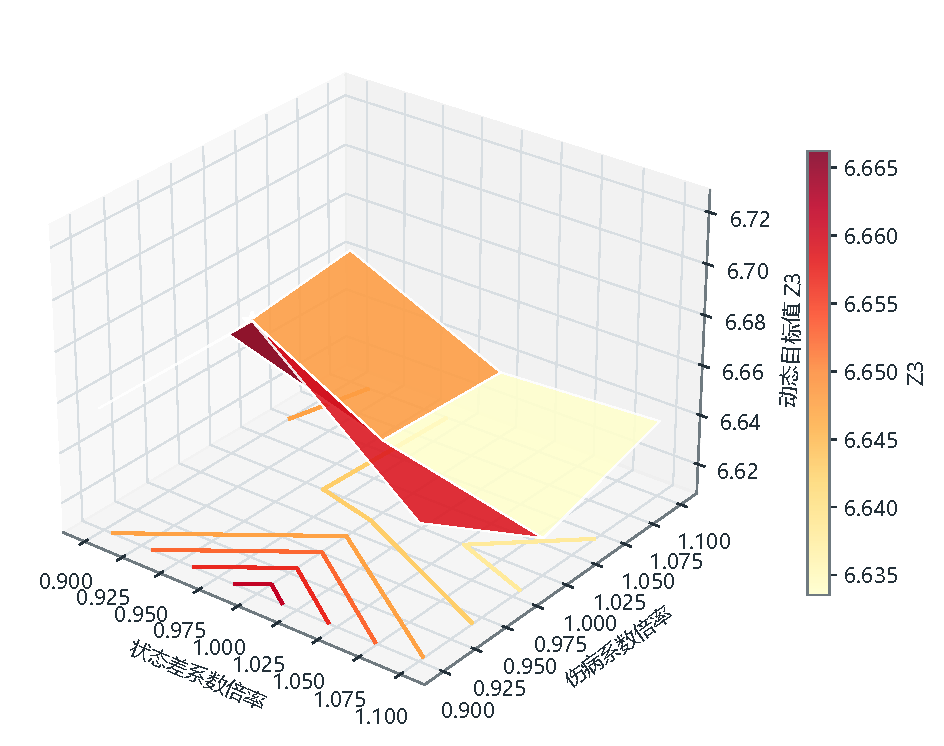
\includegraphics[width=0.76\textwidth]{figures/fig_q3_sensitivity_surface.pdf}
\caption{状态差与伤病系数下的动态目标曲面}
\label{fig:q3-sensitivity-surface}
\end{figure}

\begin{figure}[H]
\centering
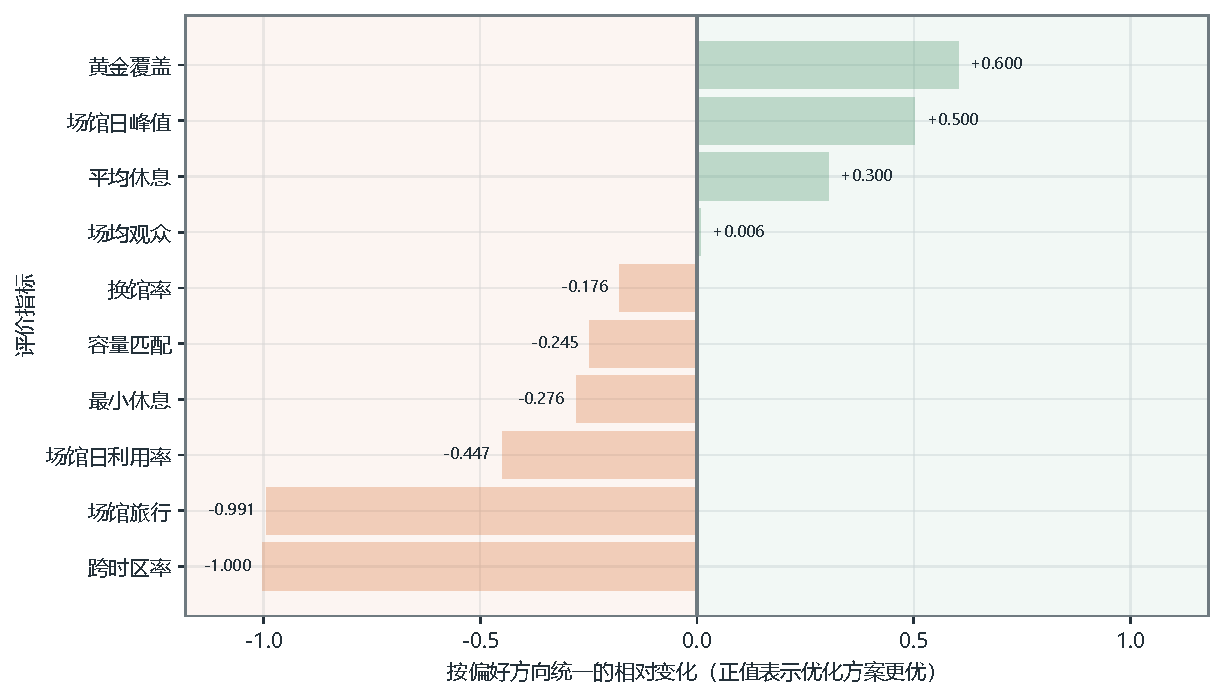
\includegraphics[width=0.88\textwidth]{figures/fig_q4_schedule_difference.pdf}
\caption{按偏好方向统一的两方案指标差异}
\label{fig:q4-schedule-difference}
\end{figure}

\begin{figure}[H]
\centering
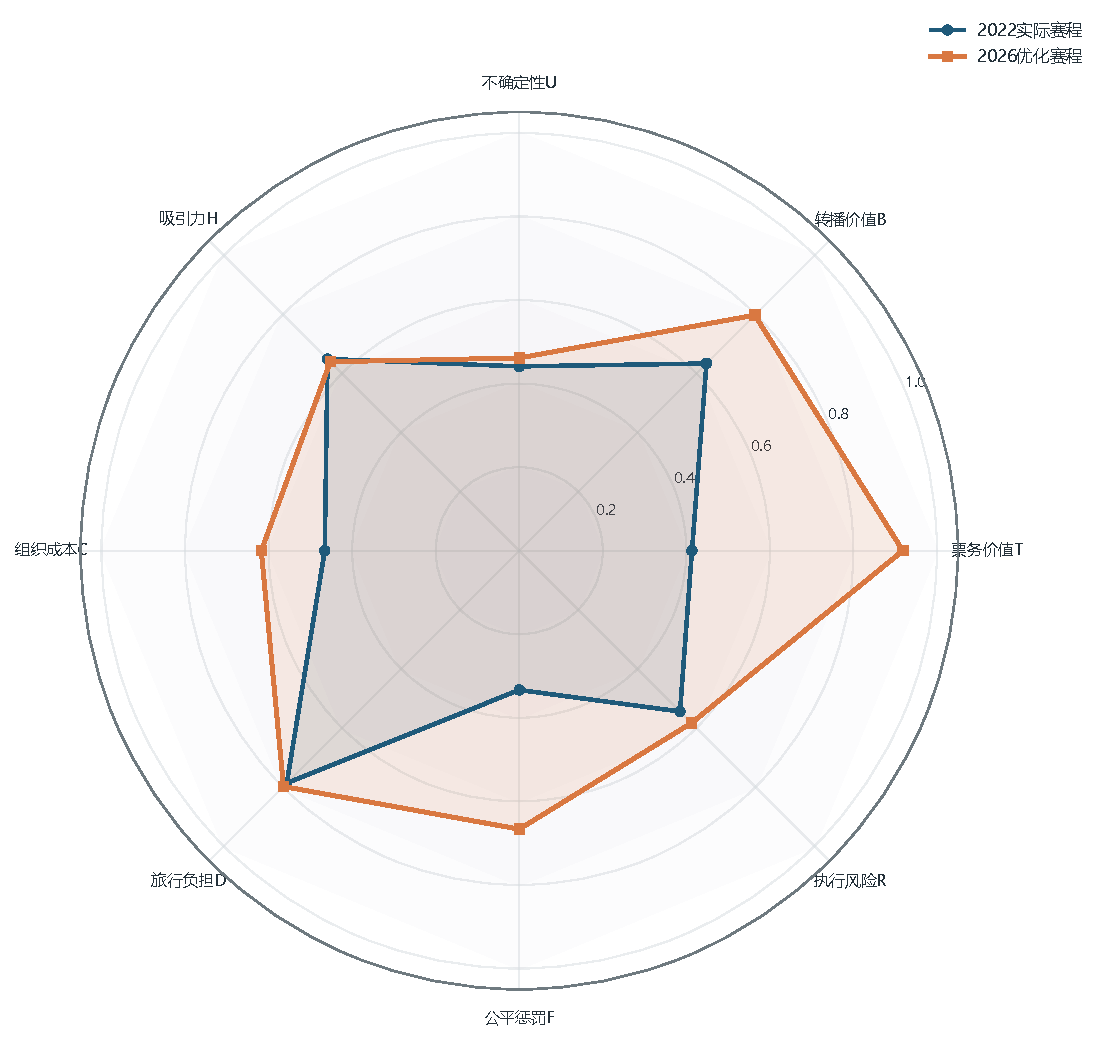
\includegraphics[width=0.72\textwidth]{figures/fig_q4_metric_radar.pdf}
\caption{实际赛程与优化赛程多维偏好得分}
\label{fig:q4-metric-radar}
\end{figure}

{
\footnotesize
\hfuzz=0.2pt
\setlength{\tabcolsep}{3pt}
\begin{longtable}{p{0.15\textwidth}p{0.16\textwidth}p{0.15\textwidth}p{0.18\textwidth}p{0.19\textwidth}}
\caption{问题一特征字典与时间血缘}\label{tab:q1-data-dictionary}\\
\toprule
特征 & 来源表 & 来源列 & 时间规则 & 拟合样本 \\
\midrule
\endfirsthead
\multicolumn{5}{c}{续表} \\
\toprule
特征 & 来源表 & 来源列 & 时间规则 & 拟合样本 \\
\midrule
\endhead
\midrule \multicolumn{5}{r}{续下页} \\
\endfoot
\bottomrule
\endlastfoot
competition & historical\_\allowbreak{}matches/\allowbreak{}teams/\allowbreak{}base\_\allowbreak{}predictions & competition & pregame\_\allowbreak{}available & outer\_\allowbreak{}fold\_\allowbreak{}train\_\allowbreak{}only;\allowbreak{} final=560 train ids \\
stage & historical\_\allowbreak{}matches/\allowbreak{}teams/\allowbreak{}base\_\allowbreak{}predictions & stage & pregame\_\allowbreak{}available & outer\_\allowbreak{}fold\_\allowbreak{}train\_\allowbreak{}only;\allowbreak{} final=560 train ids \\
timezone\_\allowbreak{}pair & historical\_\allowbreak{}matches/\allowbreak{}teams/\allowbreak{}base\_\allowbreak{}predictions & timezone\_\allowbreak{}pair & pregame\_\allowbreak{}available & outer\_\allowbreak{}fold\_\allowbreak{}train\_\allowbreak{}only;\allowbreak{} final=560 train ids \\
strength\_\allowbreak{}rank\_\allowbreak{}mean & historical\_\allowbreak{}matches/\allowbreak{}teams/\allowbreak{}base\_\allowbreak{}predictions & strength\_\allowbreak{}rank\_\allowbreak{}mean & pregame\_\allowbreak{}available & outer\_\allowbreak{}fold\_\allowbreak{}train\_\allowbreak{}only;\allowbreak{} final=560 train ids \\
strength\_\allowbreak{}rank\_\allowbreak{}gap & historical\_\allowbreak{}matches/\allowbreak{}teams/\allowbreak{}base\_\allowbreak{}predictions & strength\_\allowbreak{}rank\_\allowbreak{}gap & pregame\_\allowbreak{}available & outer\_\allowbreak{}fold\_\allowbreak{}train\_\allowbreak{}only;\allowbreak{} final=560 train ids \\
elo\_\allowbreak{}mean & historical\_\allowbreak{}matches/\allowbreak{}teams/\allowbreak{}base\_\allowbreak{}predictions & elo\_\allowbreak{}mean & pregame\_\allowbreak{}available & outer\_\allowbreak{}fold\_\allowbreak{}train\_\allowbreak{}only;\allowbreak{} final=560 train ids \\
elo\_\allowbreak{}gap & historical\_\allowbreak{}matches/\allowbreak{}teams/\allowbreak{}base\_\allowbreak{}predictions & elo\_\allowbreak{}gap & pregame\_\allowbreak{}available & outer\_\allowbreak{}fold\_\allowbreak{}train\_\allowbreak{}only;\allowbreak{} final=560 train ids \\
p\_\allowbreak{}a & historical\_\allowbreak{}matches/\allowbreak{}teams/\allowbreak{}base\_\allowbreak{}predictions & p\_\allowbreak{}a & pregame\_\allowbreak{}available & outer\_\allowbreak{}fold\_\allowbreak{}train\_\allowbreak{}only;\allowbreak{} final=560 train ids \\
p\_\allowbreak{}draw & historical\_\allowbreak{}matches/\allowbreak{}teams/\allowbreak{}base\_\allowbreak{}predictions & p\_\allowbreak{}draw & pregame\_\allowbreak{}available & outer\_\allowbreak{}fold\_\allowbreak{}train\_\allowbreak{}only;\allowbreak{} final=560 train ids \\
p\_\allowbreak{}b & historical\_\allowbreak{}matches/\allowbreak{}teams/\allowbreak{}base\_\allowbreak{}predictions & p\_\allowbreak{}b & pregame\_\allowbreak{}available & outer\_\allowbreak{}fold\_\allowbreak{}train\_\allowbreak{}only;\allowbreak{} final=560 train ids \\
odds\_\allowbreak{}entropy & historical\_\allowbreak{}matches/\allowbreak{}teams/\allowbreak{}base\_\allowbreak{}predictions & odds\_\allowbreak{}entropy & pregame\_\allowbreak{}available & outer\_\allowbreak{}fold\_\allowbreak{}train\_\allowbreak{}only;\allowbreak{} final=560 train ids \\
market\_\allowbreak{}value\_\allowbreak{}musd\_\allowbreak{}mean & historical\_\allowbreak{}matches/\allowbreak{}teams/\allowbreak{}base\_\allowbreak{}predictions & market\_\allowbreak{}value\_\allowbreak{}musd\_\allowbreak{}mean & pregame\_\allowbreak{}available & outer\_\allowbreak{}fold\_\allowbreak{}train\_\allowbreak{}only;\allowbreak{} final=560 train ids \\
market\_\allowbreak{}value\_\allowbreak{}musd\_\allowbreak{}gap & historical\_\allowbreak{}matches/\allowbreak{}teams/\allowbreak{}base\_\allowbreak{}predictions & market\_\allowbreak{}value\_\allowbreak{}musd\_\allowbreak{}gap & pregame\_\allowbreak{}available & outer\_\allowbreak{}fold\_\allowbreak{}train\_\allowbreak{}only;\allowbreak{} final=560 train ids \\
avg\_\allowbreak{}age\_\allowbreak{}mean & historical\_\allowbreak{}matches/\allowbreak{}teams/\allowbreak{}base\_\allowbreak{}predictions & avg\_\allowbreak{}age\_\allowbreak{}mean & pregame\_\allowbreak{}available & outer\_\allowbreak{}fold\_\allowbreak{}train\_\allowbreak{}only;\allowbreak{} final=560 train ids \\
avg\_\allowbreak{}age\_\allowbreak{}gap & historical\_\allowbreak{}matches/\allowbreak{}teams/\allowbreak{}base\_\allowbreak{}predictions & avg\_\allowbreak{}age\_\allowbreak{}gap & pregame\_\allowbreak{}available & outer\_\allowbreak{}fold\_\allowbreak{}train\_\allowbreak{}only;\allowbreak{} final=560 train ids \\
star\_\allowbreak{}index\_\allowbreak{}mean & historical\_\allowbreak{}matches/\allowbreak{}teams/\allowbreak{}base\_\allowbreak{}predictions & star\_\allowbreak{}index\_\allowbreak{}mean & pregame\_\allowbreak{}available & outer\_\allowbreak{}fold\_\allowbreak{}train\_\allowbreak{}only;\allowbreak{} final=560 train ids \\
star\_\allowbreak{}index\_\allowbreak{}gap & historical\_\allowbreak{}matches/\allowbreak{}teams/\allowbreak{}base\_\allowbreak{}predictions & star\_\allowbreak{}index\_\allowbreak{}gap & pregame\_\allowbreak{}available & outer\_\allowbreak{}fold\_\allowbreak{}train\_\allowbreak{}only;\allowbreak{} final=560 train ids \\
fan\_\allowbreak{}base\_\allowbreak{}index\_\allowbreak{}mean & historical\_\allowbreak{}matches/\allowbreak{}teams/\allowbreak{}base\_\allowbreak{}predictions & fan\_\allowbreak{}base\_\allowbreak{}index\_\allowbreak{}mean & pregame\_\allowbreak{}available & outer\_\allowbreak{}fold\_\allowbreak{}train\_\allowbreak{}only;\allowbreak{} final=560 train ids \\
fan\_\allowbreak{}base\_\allowbreak{}index\_\allowbreak{}gap & historical\_\allowbreak{}matches/\allowbreak{}teams/\allowbreak{}base\_\allowbreak{}predictions & fan\_\allowbreak{}base\_\allowbreak{}index\_\allowbreak{}gap & pregame\_\allowbreak{}available & outer\_\allowbreak{}fold\_\allowbreak{}train\_\allowbreak{}only;\allowbreak{} final=560 train ids \\
style\_\allowbreak{}attack\_\allowbreak{}mean & historical\_\allowbreak{}matches/\allowbreak{}teams/\allowbreak{}base\_\allowbreak{}predictions & style\_\allowbreak{}attack\_\allowbreak{}mean & pregame\_\allowbreak{}available & outer\_\allowbreak{}fold\_\allowbreak{}train\_\allowbreak{}only;\allowbreak{} final=560 train ids \\
style\_\allowbreak{}attack\_\allowbreak{}gap & historical\_\allowbreak{}matches/\allowbreak{}teams/\allowbreak{}base\_\allowbreak{}predictions & style\_\allowbreak{}attack\_\allowbreak{}gap & pregame\_\allowbreak{}available & outer\_\allowbreak{}fold\_\allowbreak{}train\_\allowbreak{}only;\allowbreak{} final=560 train ids \\
style\_\allowbreak{}defense\_\allowbreak{}mean & historical\_\allowbreak{}matches/\allowbreak{}teams/\allowbreak{}base\_\allowbreak{}predictions & style\_\allowbreak{}defense\_\allowbreak{}mean & pregame\_\allowbreak{}available & outer\_\allowbreak{}fold\_\allowbreak{}train\_\allowbreak{}only;\allowbreak{} final=560 train ids \\
style\_\allowbreak{}defense\_\allowbreak{}gap & historical\_\allowbreak{}matches/\allowbreak{}teams/\allowbreak{}base\_\allowbreak{}predictions & style\_\allowbreak{}defense\_\allowbreak{}gap & pregame\_\allowbreak{}available & outer\_\allowbreak{}fold\_\allowbreak{}train\_\allowbreak{}only;\allowbreak{} final=560 train ids \\
host\_\allowbreak{}flag\_\allowbreak{}mean & historical\_\allowbreak{}matches/\allowbreak{}teams/\allowbreak{}base\_\allowbreak{}predictions & host\_\allowbreak{}flag\_\allowbreak{}mean & pregame\_\allowbreak{}available & outer\_\allowbreak{}fold\_\allowbreak{}train\_\allowbreak{}only;\allowbreak{} final=560 train ids \\
host\_\allowbreak{}flag\_\allowbreak{}gap & historical\_\allowbreak{}matches/\allowbreak{}teams/\allowbreak{}base\_\allowbreak{}predictions & host\_\allowbreak{}flag\_\allowbreak{}gap & pregame\_\allowbreak{}available & outer\_\allowbreak{}fold\_\allowbreak{}train\_\allowbreak{}only;\allowbreak{} final=560 train ids \\
strength\_\allowbreak{}score\_\allowbreak{}mean & historical\_\allowbreak{}matches/\allowbreak{}teams/\allowbreak{}base\_\allowbreak{}predictions & strength\_\allowbreak{}score\_\allowbreak{}mean & pregame\_\allowbreak{}available & outer\_\allowbreak{}fold\_\allowbreak{}train\_\allowbreak{}only;\allowbreak{} final=560 train ids \\
strength\_\allowbreak{}score\_\allowbreak{}gap & historical\_\allowbreak{}matches/\allowbreak{}teams/\allowbreak{}base\_\allowbreak{}predictions & strength\_\allowbreak{}score\_\allowbreak{}gap & pregame\_\allowbreak{}available & outer\_\allowbreak{}fold\_\allowbreak{}train\_\allowbreak{}only;\allowbreak{} final=560 train ids \\
a\_\allowbreak{}hist\_\allowbreak{}goals\_\allowbreak{}roll5 & historical\_\allowbreak{}matches & a\_\allowbreak{}hist\_\allowbreak{}goals\_\allowbreak{}roll5 & strictly\_\allowbreak{}before\_\allowbreak{}kickoff\_\allowbreak{}shift1 & outer\_\allowbreak{}fold\_\allowbreak{}train\_\allowbreak{}only;\allowbreak{} final=560 train ids \\
a\_\allowbreak{}hist\_\allowbreak{}goals\_\allowbreak{}ewm5 & historical\_\allowbreak{}matches & a\_\allowbreak{}hist\_\allowbreak{}goals\_\allowbreak{}ewm5 & strictly\_\allowbreak{}before\_\allowbreak{}kickoff\_\allowbreak{}shift1 & outer\_\allowbreak{}fold\_\allowbreak{}train\_\allowbreak{}only;\allowbreak{} final=560 train ids \\
a\_\allowbreak{}hist\_\allowbreak{}xg\_\allowbreak{}roll5 & historical\_\allowbreak{}matches & a\_\allowbreak{}hist\_\allowbreak{}xg\_\allowbreak{}roll5 & strictly\_\allowbreak{}before\_\allowbreak{}kickoff\_\allowbreak{}shift1 & outer\_\allowbreak{}fold\_\allowbreak{}train\_\allowbreak{}only;\allowbreak{} final=560 train ids \\
a\_\allowbreak{}hist\_\allowbreak{}xg\_\allowbreak{}ewm5 & historical\_\allowbreak{}matches & a\_\allowbreak{}hist\_\allowbreak{}xg\_\allowbreak{}ewm5 & strictly\_\allowbreak{}before\_\allowbreak{}kickoff\_\allowbreak{}shift1 & outer\_\allowbreak{}fold\_\allowbreak{}train\_\allowbreak{}only;\allowbreak{} final=560 train ids \\
a\_\allowbreak{}hist\_\allowbreak{}shots\_\allowbreak{}roll5 & historical\_\allowbreak{}matches & a\_\allowbreak{}hist\_\allowbreak{}shots\_\allowbreak{}roll5 & strictly\_\allowbreak{}before\_\allowbreak{}kickoff\_\allowbreak{}shift1 & outer\_\allowbreak{}fold\_\allowbreak{}train\_\allowbreak{}only;\allowbreak{} final=560 train ids \\
a\_\allowbreak{}hist\_\allowbreak{}shots\_\allowbreak{}ewm5 & historical\_\allowbreak{}matches & a\_\allowbreak{}hist\_\allowbreak{}shots\_\allowbreak{}ewm5 & strictly\_\allowbreak{}before\_\allowbreak{}kickoff\_\allowbreak{}shift1 & outer\_\allowbreak{}fold\_\allowbreak{}train\_\allowbreak{}only;\allowbreak{} final=560 train ids \\
a\_\allowbreak{}hist\_\allowbreak{}possession\_\allowbreak{}roll5 & historical\_\allowbreak{}matches & a\_\allowbreak{}hist\_\allowbreak{}possession\_\allowbreak{}roll5 & strictly\_\allowbreak{}before\_\allowbreak{}kickoff\_\allowbreak{}shift1 & outer\_\allowbreak{}fold\_\allowbreak{}train\_\allowbreak{}only;\allowbreak{} final=560 train ids \\
a\_\allowbreak{}hist\_\allowbreak{}possession\_\allowbreak{}ewm5 & historical\_\allowbreak{}matches & a\_\allowbreak{}hist\_\allowbreak{}possession\_\allowbreak{}ewm5 & strictly\_\allowbreak{}before\_\allowbreak{}kickoff\_\allowbreak{}shift1 & outer\_\allowbreak{}fold\_\allowbreak{}train\_\allowbreak{}only;\allowbreak{} final=560 train ids \\
a\_\allowbreak{}hist\_\allowbreak{}attendance\_\allowbreak{}roll5 & historical\_\allowbreak{}matches & a\_\allowbreak{}hist\_\allowbreak{}attendance\_\allowbreak{}roll5 & strictly\_\allowbreak{}before\_\allowbreak{}kickoff\_\allowbreak{}shift1 & outer\_\allowbreak{}fold\_\allowbreak{}train\_\allowbreak{}only;\allowbreak{} final=560 train ids \\
a\_\allowbreak{}hist\_\allowbreak{}attendance\_\allowbreak{}ewm5 & historical\_\allowbreak{}matches & a\_\allowbreak{}hist\_\allowbreak{}attendance\_\allowbreak{}ewm5 & strictly\_\allowbreak{}before\_\allowbreak{}kickoff\_\allowbreak{}shift1 & outer\_\allowbreak{}fold\_\allowbreak{}train\_\allowbreak{}only;\allowbreak{} final=560 train ids \\
a\_\allowbreak{}hist\_\allowbreak{}tv\_\allowbreak{}viewers\_\allowbreak{}roll5 & historical\_\allowbreak{}matches & a\_\allowbreak{}hist\_\allowbreak{}tv\_\allowbreak{}viewers\_\allowbreak{}roll5 & strictly\_\allowbreak{}before\_\allowbreak{}kickoff\_\allowbreak{}shift1 & outer\_\allowbreak{}fold\_\allowbreak{}train\_\allowbreak{}only;\allowbreak{} final=560 train ids \\
a\_\allowbreak{}hist\_\allowbreak{}tv\_\allowbreak{}viewers\_\allowbreak{}ewm5 & historical\_\allowbreak{}matches & a\_\allowbreak{}hist\_\allowbreak{}tv\_\allowbreak{}viewers\_\allowbreak{}ewm5 & strictly\_\allowbreak{}before\_\allowbreak{}kickoff\_\allowbreak{}shift1 & outer\_\allowbreak{}fold\_\allowbreak{}train\_\allowbreak{}only;\allowbreak{} final=560 train ids \\
b\_\allowbreak{}hist\_\allowbreak{}goals\_\allowbreak{}roll5 & historical\_\allowbreak{}matches & b\_\allowbreak{}hist\_\allowbreak{}goals\_\allowbreak{}roll5 & strictly\_\allowbreak{}before\_\allowbreak{}kickoff\_\allowbreak{}shift1 & outer\_\allowbreak{}fold\_\allowbreak{}train\_\allowbreak{}only;\allowbreak{} final=560 train ids \\
b\_\allowbreak{}hist\_\allowbreak{}goals\_\allowbreak{}ewm5 & historical\_\allowbreak{}matches & b\_\allowbreak{}hist\_\allowbreak{}goals\_\allowbreak{}ewm5 & strictly\_\allowbreak{}before\_\allowbreak{}kickoff\_\allowbreak{}shift1 & outer\_\allowbreak{}fold\_\allowbreak{}train\_\allowbreak{}only;\allowbreak{} final=560 train ids \\
b\_\allowbreak{}hist\_\allowbreak{}xg\_\allowbreak{}roll5 & historical\_\allowbreak{}matches & b\_\allowbreak{}hist\_\allowbreak{}xg\_\allowbreak{}roll5 & strictly\_\allowbreak{}before\_\allowbreak{}kickoff\_\allowbreak{}shift1 & outer\_\allowbreak{}fold\_\allowbreak{}train\_\allowbreak{}only;\allowbreak{} final=560 train ids \\
b\_\allowbreak{}hist\_\allowbreak{}xg\_\allowbreak{}ewm5 & historical\_\allowbreak{}matches & b\_\allowbreak{}hist\_\allowbreak{}xg\_\allowbreak{}ewm5 & strictly\_\allowbreak{}before\_\allowbreak{}kickoff\_\allowbreak{}shift1 & outer\_\allowbreak{}fold\_\allowbreak{}train\_\allowbreak{}only;\allowbreak{} final=560 train ids \\
b\_\allowbreak{}hist\_\allowbreak{}shots\_\allowbreak{}roll5 & historical\_\allowbreak{}matches & b\_\allowbreak{}hist\_\allowbreak{}shots\_\allowbreak{}roll5 & strictly\_\allowbreak{}before\_\allowbreak{}kickoff\_\allowbreak{}shift1 & outer\_\allowbreak{}fold\_\allowbreak{}train\_\allowbreak{}only;\allowbreak{} final=560 train ids \\
b\_\allowbreak{}hist\_\allowbreak{}shots\_\allowbreak{}ewm5 & historical\_\allowbreak{}matches & b\_\allowbreak{}hist\_\allowbreak{}shots\_\allowbreak{}ewm5 & strictly\_\allowbreak{}before\_\allowbreak{}kickoff\_\allowbreak{}shift1 & outer\_\allowbreak{}fold\_\allowbreak{}train\_\allowbreak{}only;\allowbreak{} final=560 train ids \\
b\_\allowbreak{}hist\_\allowbreak{}possession\_\allowbreak{}roll5 & historical\_\allowbreak{}matches & b\_\allowbreak{}hist\_\allowbreak{}possession\_\allowbreak{}roll5 & strictly\_\allowbreak{}before\_\allowbreak{}kickoff\_\allowbreak{}shift1 & outer\_\allowbreak{}fold\_\allowbreak{}train\_\allowbreak{}only;\allowbreak{} final=560 train ids \\
b\_\allowbreak{}hist\_\allowbreak{}possession\_\allowbreak{}ewm5 & historical\_\allowbreak{}matches & b\_\allowbreak{}hist\_\allowbreak{}possession\_\allowbreak{}ewm5 & strictly\_\allowbreak{}before\_\allowbreak{}kickoff\_\allowbreak{}shift1 & outer\_\allowbreak{}fold\_\allowbreak{}train\_\allowbreak{}only;\allowbreak{} final=560 train ids \\
b\_\allowbreak{}hist\_\allowbreak{}attendance\_\allowbreak{}roll5 & historical\_\allowbreak{}matches & b\_\allowbreak{}hist\_\allowbreak{}attendance\_\allowbreak{}roll5 & strictly\_\allowbreak{}before\_\allowbreak{}kickoff\_\allowbreak{}shift1 & outer\_\allowbreak{}fold\_\allowbreak{}train\_\allowbreak{}only;\allowbreak{} final=560 train ids \\
b\_\allowbreak{}hist\_\allowbreak{}attendance\_\allowbreak{}ewm5 & historical\_\allowbreak{}matches & b\_\allowbreak{}hist\_\allowbreak{}attendance\_\allowbreak{}ewm5 & strictly\_\allowbreak{}before\_\allowbreak{}kickoff\_\allowbreak{}shift1 & outer\_\allowbreak{}fold\_\allowbreak{}train\_\allowbreak{}only;\allowbreak{} final=560 train ids \\
b\_\allowbreak{}hist\_\allowbreak{}tv\_\allowbreak{}viewers\_\allowbreak{}roll5 & historical\_\allowbreak{}matches & b\_\allowbreak{}hist\_\allowbreak{}tv\_\allowbreak{}viewers\_\allowbreak{}roll5 & strictly\_\allowbreak{}before\_\allowbreak{}kickoff\_\allowbreak{}shift1 & outer\_\allowbreak{}fold\_\allowbreak{}train\_\allowbreak{}only;\allowbreak{} final=560 train ids \\
b\_\allowbreak{}hist\_\allowbreak{}tv\_\allowbreak{}viewers\_\allowbreak{}ewm5 & historical\_\allowbreak{}matches & b\_\allowbreak{}hist\_\allowbreak{}tv\_\allowbreak{}viewers\_\allowbreak{}ewm5 & strictly\_\allowbreak{}before\_\allowbreak{}kickoff\_\allowbreak{}shift1 & outer\_\allowbreak{}fold\_\allowbreak{}train\_\allowbreak{}only;\allowbreak{} final=560 train ids \\
worldcup\_\allowbreak{}stage & historical\_\allowbreak{}matches/\allowbreak{}teams/\allowbreak{}base\_\allowbreak{}predictions & worldcup\_\allowbreak{}stage & pregame\_\allowbreak{}available & outer\_\allowbreak{}fold\_\allowbreak{}train\_\allowbreak{}only;\allowbreak{} final=560 train ids \\
fan\_\allowbreak{}stage\_\allowbreak{}interaction & historical\_\allowbreak{}matches/\allowbreak{}teams/\allowbreak{}base\_\allowbreak{}predictions & fan\_\allowbreak{}stage\_\allowbreak{}interaction & pregame\_\allowbreak{}available & outer\_\allowbreak{}fold\_\allowbreak{}train\_\allowbreak{}only;\allowbreak{} final=560 train ids \\
star\_\allowbreak{}stage\_\allowbreak{}interaction & historical\_\allowbreak{}matches/\allowbreak{}teams/\allowbreak{}base\_\allowbreak{}predictions & star\_\allowbreak{}stage\_\allowbreak{}interaction & pregame\_\allowbreak{}available & outer\_\allowbreak{}fold\_\allowbreak{}train\_\allowbreak{}only;\allowbreak{} final=560 train ids \\
strength\_\allowbreak{}entropy\_\allowbreak{}interaction & historical\_\allowbreak{}matches/\allowbreak{}teams/\allowbreak{}base\_\allowbreak{}predictions & strength\_\allowbreak{}entropy\_\allowbreak{}interaction & pregame\_\allowbreak{}available & outer\_\allowbreak{}fold\_\allowbreak{}train\_\allowbreak{}only;\allowbreak{} final=560 train ids \\
\end{longtable}
\par
}

\begin{table}[H]
\centering
\caption{问题一时序交叉验证误差}
\label{tab:q1-model-metrics}
\small
\resizebox{\textwidth}{!}{%
\begin{tabular}{llrrrrr}
\toprule
模型 & 窗口 & MSE & RMSE & MAE & 训练截至 & 验证起始 \\
\midrule
MeanBaseline & 折1 & 598.919 & 24.473 & 19.751 & 2019-01-26 & 2019-02-03 \\
ElasticNet & 折1 & 243.138 & 15.593 & 12.757 & 2019-01-26 & 2019-02-03 \\
ExtraTrees & 折1 & 298.141 & 17.267 & 14.214 & 2019-01-26 & 2019-02-03 \\
CatBoost & 折1 & 274.080 & 16.555 & 13.172 & 2019-01-26 & 2019-02-03 \\
MeanBaseline & 折2 & 621.856 & 24.937 & 19.817 & 2020-03-29 & 2020-04-04 \\
ElasticNet & 折2 & 226.619 & 15.054 & 11.929 & 2020-03-29 & 2020-04-04 \\
ExtraTrees & 折2 & 261.458 & 16.170 & 12.694 & 2020-03-29 & 2020-04-04 \\
CatBoost & 折2 & 244.634 & 15.641 & 12.265 & 2020-03-29 & 2020-04-04 \\
MeanBaseline & 折3 & 528.105 & 22.981 & 18.864 & 2021-04-19 & 2021-04-22 \\
ElasticNet & 折3 & 239.340 & 15.471 & 12.203 & 2021-04-19 & 2021-04-22 \\
ExtraTrees & 折3 & 256.627 & 16.020 & 13.012 & 2021-04-19 & 2021-04-22 \\
CatBoost & 折3 & 243.231 & 15.596 & 12.693 & 2021-04-19 & 2021-04-22 \\
MeanBaseline & 折4 & 575.265 & 23.985 & 18.588 & 2022-07-03 & 2022-07-05 \\
ElasticNet & 折4 & 214.684 & 14.652 & 11.510 & 2022-07-03 & 2022-07-05 \\
ExtraTrees & 折4 & 242.182 & 15.562 & 12.326 & 2022-07-03 & 2022-07-05 \\
CatBoost & 折4 & 230.889 & 15.195 & 11.874 & 2022-07-03 & 2022-07-05 \\
MeanBaseline & 折5 & 581.872 & 24.122 & 19.646 & 2023-07-28 & 2023-07-29 \\
ElasticNet & 折5 & 176.646 & 13.291 & 10.739 & 2023-07-28 & 2023-07-29 \\
ExtraTrees & 折5 & 192.403 & 13.871 & 11.426 & 2023-07-28 & 2023-07-29 \\
CatBoost & 折5 & 178.211 & 13.350 & 10.915 & 2023-07-28 & 2023-07-29 \\
ElasticNet & 总体均值 & 220.086 & 14.812 & 11.828 & -- & -- \\
CatBoost & 总体均值 & 234.209 & 15.267 & 12.184 & -- & -- \\
ExtraTrees & 总体均值 & 250.162 & 15.778 & 12.734 & -- & -- \\
MeanBaseline & 总体均值 & 581.203 & 24.099 & 19.333 & -- & -- \\
\bottomrule
\end{tabular}
}
\vspace{2pt}
\noindent\begin{minipage}{0.96\textwidth}\footnotesize 注：误差单位为百万人口径；最终选择模型为 ElasticNet。\end{minipage}
\end{table}

\begin{table}[H]
\centering
\caption{问题一核心变量描述性统计}
\label{tab:q1-descriptive}
\small
\resizebox{\textwidth}{!}{%
\begin{tabular}{lrrrrrrrr}
\toprule
变量 & 样本数 & 均值 & 标准差 & 最小值 & P25 & 中位数 & P75 & 最大值 \\
\midrule
观看人数 & 560 & 145.64 & 23.56 & 93.96 & 128.43 & 142.11 & 160.62 & 225.41 \\
平均Elo & 560 & 1756.86 & 120.58 & 1472.50 & 1671.00 & 1758.00 & 1846.50 & 2025.50 \\
平均排名 & 560 & 24.30 & 9.97 & 2.50 & 17.00 & 24.00 & 31.50 & 47.50 \\
平均球迷基础 & 560 & 73.41 & 10.47 & 46.30 & 66.05 & 73.03 & 81.93 & 94.40 \\
赔率熵 & 560 & 1.00 & 0.10 & 0.71 & 0.95 & 1.04 & 1.08 & 1.10 \\
\bottomrule
\end{tabular}
}
\vspace{2pt}
\noindent\begin{minipage}{0.96\textwidth}\footnotesize 注：观看人数单位为百万人；其余变量采用源数据或赛前构造口径。\end{minipage}
\end{table}

\begin{table}[H]
\centering
\caption{问题二关键约束复算与裕度}
\label{tab:q2-constraint-audit}
\small
\begin{tabular}{lrrrrc}
\toprule
约束族 & 实际值 & 界值 & 单位 & 最小裕度 & 状态 \\
\midrule
最小轮间休息 & 63.000 & 60.000 & 小时 & 5.0\% & 通过 \\
场馆承办下界 & 0.000 & 0.000 & 剩余场 & 0.0\% & 通过 \\
场馆承办上界 & 0.000 & 0.000 & 剩余场 & 0.0\% & 通过 \\
场馆单日本地容量 & 1.000 & 1.000 & 最大利用率 & 0.0\% & 通过 \\
场馆安保等级 & 0.000 & 0.000 & 等级余量 & 0.0\% & 通过 \\
时段转播容量 & 0.000 & 0.000 & 剩余场 & 0.0\% & 通过 \\
第三轮高安保日容量 & 0.000 & 0.000 & 比例余量 & 0.0\% & 通过 \\
黄金时段公平极差 & 1.000 & 2.000 & 场 & 50.0\% & 通过 \\
\bottomrule
\end{tabular}
\vspace{2pt}
\noindent\begin{minipage}{0.96\textwidth}\footnotesize 注：裕度为按各约束自身上限归一化后的最小剩余比例；零表示约束在最紧样本上取等。\end{minipage}
\end{table}

\begin{table}[H]
\centering
\caption{问题二场馆负载与赛程汇总}
\label{tab:q2-schedule-summary}
\small
\resizebox{\textwidth}{!}{%
\begin{tabular}{llrrrr}
\toprule
场馆 & 城市 & 场次 & 黄金时段场次 & 平均旅行指数 & 预计观众合计（万人） \\
\midrule
V01 & Atlanta & 8 & 4 & 0.254 & 32.6 \\
V02 & Boston & 8 & 5 & 0.321 & 30.0 \\
V03 & Dallas & 7 & 7 & 0.081 & 27.1 \\
V04 & Guadalajara & 8 & 6 & 0.152 & 35.1 \\
V05 & Houston & 8 & 6 & 0.086 & 35.2 \\
V06 & Kansas City & 5 & 5 & 0.086 & 17.3 \\
V07 & Los Angeles & 4 & 1 & 0.270 & 16.7 \\
V08 & Mexico City & 7 & 7 & 0.110 & 34.3 \\
V09 & Miami & 3 & 1 & 0.244 & 13.9 \\
V10 & Monterrey & 2 & 0 & 0.096 & 6.7 \\
V11 & New York/New Jersey & 2 & 1 & 0.117 & 6.9 \\
V12 & Philadelphia & 2 & 1 & 0.272 & 9.3 \\
V13 & San Francisco Bay Area & 2 & 1 & 0.414 & 9.0 \\
V14 & Seattle & 2 & 0 & 0.556 & 8.4 \\
V15 & Toronto & 2 & 0 & 0.266 & 8.5 \\
V16 & Vancouver & 2 & 0 & 0.504 & 9.4 \\
\bottomrule
\end{tabular}
}
\vspace{2pt}
\noindent\begin{minipage}{0.96\textwidth}\footnotesize 注：主方案 Z2=0.484946，最小轮间休息 63 小时。\end{minipage}
\end{table}

\begin{table}[H]
\centering
\caption{问题三晋级概率、条件概率与风险}
\label{tab:q3-probability-risk}
\small
\resizebox{\textwidth}{!}{%
\begin{tabular}{llrlrrrrr}
\toprule
比赛 & A队 & A队晋级 & B队 & B队晋级 & A胜条件晋级 & B胜条件晋级 & 无悬念风险 & 默契风险 \\
\midrule
GA05 & Mexico & 1.000 & Czechia & 1.000 & 1.000 & 1.000 & 1.000 & 0.650 \\
GA06 & South Africa & 0.226 & South Korea & 0.541 & 1.000 & 0.991 & 0.154 & 0.000 \\
GB05 & Canada & 0.355 & Switzerland & 1.000 & 1.000 & 1.000 & 0.542 & 0.803 \\
GB06 & Bosnia and Herzegovina & 0.601 & Qatar & 0.318 & 1.000 & 1.000 & 0.087 & 0.013 \\
GC05 & Brazil & 1.000 & Scotland & 0.077 & 1.000 & 1.000 & 0.857 & 0.015 \\
GC06 & Morocco & 0.963 & Haiti & 0.209 & 1.000 & 1.000 & 0.599 & 0.704 \\
GD05 & United States & 1.000 & Turkey & 1.000 & 1.000 & 1.000 & 1.000 & 0.650 \\
GD06 & Paraguay & 0.314 & Australia & 0.631 & 0.851 & 1.000 & 0.103 & 0.000 \\
GE05 & Germany & 1.000 & Ecuador & 0.954 & 1.000 & 1.000 & 0.912 & 0.681 \\
GE06 & Curacao & 0.002 & Ivory Coast & 1.000 & 0.021 & 1.000 & 0.995 & 0.000 \\
GF05 & Netherlands & 1.000 & Tunisia & 0.070 & 1.000 & 1.000 & 0.870 & 0.002 \\
GF06 & Japan & 0.934 & Sweden & 0.319 & 1.000 & 1.000 & 0.442 & 0.001 \\
GG05 & Belgium & 1.000 & New Zealand & 0.782 & 1.000 & 1.000 & 0.659 & 0.769 \\
GG06 & Egypt & 0.808 & Iran & 0.155 & 1.000 & 0.416 & 0.428 & 0.000 \\
GH05 & Spain & 1.000 & Uruguay & 0.986 & 1.000 & 1.000 & 0.972 & 0.660 \\
GH06 & Cape Verde & 0.025 & Saudi Arabia & 0.965 & 0.100 & 1.000 & 0.885 & 0.000 \\
GI05 & France & 1.000 & Norway & 1.000 & 1.000 & 1.000 & 1.000 & 0.650 \\
GI06 & Senegal & 0.886 & Iraq & 0.056 & 1.000 & 0.496 & 0.692 & 0.000 \\
GJ05 & Argentina & 1.000 & Jordan & 1.000 & 1.000 & 1.000 & 1.000 & 0.650 \\
GJ06 & Algeria & 0.220 & Austria & 0.510 & 0.986 & 0.995 & 0.157 & 0.000 \\
GK05 & Portugal & 1.000 & Colombia & 1.000 & 1.000 & 1.000 & 1.000 & 0.650 \\
GK06 & DR Congo & 0.288 & Uzbekistan & 0.122 & 0.956 & 0.292 & 0.375 & 0.000 \\
GL05 & England & 1.000 & Panama & 0.588 & 1.000 & 1.000 & 0.516 & 0.820 \\
GL06 & Croatia & 1.000 & Ghana & 0.093 & 1.000 & 0.614 & 0.832 & 0.000 \\
\bottomrule
\end{tabular}
}
\vspace{2pt}
\noindent\begin{minipage}{0.96\textwidth}\footnotesize 注：条件晋级概率来自同一 20000 次联合蒙特卡洛样本，晋级名额质量守恒为每次 32 队。\end{minipage}
\end{table}

\begin{table}[H]
\centering
\caption{问题三逐日动态资源使用与容量}
\label{tab:q3-resource-budget}
\small
\resizebox{\textwidth}{!}{%
\begin{tabular}{lrrrrrrrrc}
\toprule
日期 & 高转播 & 转播上限 & 高安保 & 安保上限 & 强化交通 & 交通上限 & 预算使用 & 预算上限 & 状态 \\
\midrule
2026-06-20 & 2 & 4 & 1 & 3 & 2 & 4 & 35.0 & 120 & 通过 \\
2026-06-22 & 1 & 3 & 0 & 3 & 0 & 3 & 13.0 & 100 & 通过 \\
2026-06-23 & 3 & 3 & 3 & 3 & 3 & 3 & 86.0 & 100 & 通过 \\
2026-06-24 & 3 & 3 & 1 & 2 & 3 & 3 & 51.0 & 100 & 通过 \\
2026-06-28 & 4 & 4 & 3 & 3 & 4 & 4 & 77.0 & 120 & 通过 \\
2026-06-29 & 3 & 3 & 2 & 2 & 2 & 3 & 54.0 & 100 & 通过 \\
2026-06-30 & 3 & 3 & 2 & 2 & 3 & 3 & 59.0 & 100 & 通过 \\
\bottomrule
\end{tabular}
}
\end{table}

\begin{table}[H]
\centering
\caption{问题三静态策略与动态重优化同界比较}
\label{tab:q3-static-dynamic}
\small
\begin{tabular}{lrrrr}
\toprule
指标 & 静态策略重评 & 动态重优化 & 偏好方向改善 & 单位 \\
\midrule
票务价值 TV & 113.715 & 113.385 & -0.330 & 百万美元 \\
转播价值 BV & 168.309 & 168.368 & 0.059 & 百万美元 \\
吸引力 A & 0.512 & 0.512 & 0.000 & 无量纲 \\
资源成本 C & 396.000 & 375.000 & 21.000 & 成本指数 \\
风险 R & 0.465 & 0.469 & -0.004 & 无量纲 \\
综合目标 Z3 & 6.572230 & 6.637484 & 0.065254 & 无量纲 \\
\bottomrule
\end{tabular}
\vspace{2pt}
\noindent\begin{minipage}{0.96\textwidth}\footnotesize 注：正的偏好方向改善表示动态方案更优；成本与风险按越低越优转换。\end{minipage}
\end{table}

\begin{table}[H]
\centering
\caption{两套赛程的可观测结构与规模强度比较}
\label{tab:q4-structural-comparison}
\small
\resizebox{\textwidth}{!}{%
\begin{tabular}{lllrrl}
\toprule
指标 & 定义与分母 & 单位 & 2022实际 & 2026优化 & 偏好方向 \\
\midrule
最小休息 & 球队相邻比赛 UTC 间隔的最小值 & 小时 & 87.0000 & 63.0000 & 越高越优 \\
平均休息 & 球队相邻比赛 UTC 间隔的平均值 & 小时 & 97.8125 & 139.8125 & 越高越优 \\
跨时区次数 & 相邻比赛场馆 UTC 偏移发生变化的次数 & 次 & 0 & 78 & 越低越优 \\
跨时区率 & 跨时区次数除以球队转场次数 & 比例 & 0.0000 & 81.2500 & 越低越优 \\
场馆旅行 & 相邻比赛实际场馆大圆距离的平均值 & 公里/次 & 18.9868 & 2019.1075 & 越低越优 \\
换馆率 & 相邻轮更换场馆的球队转场比例 & 比例 & 78.1250 & 94.7917 & 越低越优 \\
场馆日利用率 & 发生比赛的场馆日占可用场馆日比例 & 比例 & 45.1923 & 25.0000 & 越高越优 \\
场馆日峰值 & 单一场馆单日承办场次最大值 & 场/场馆日 & 2 & 1 & 越低越优 \\
容量匹配 & 预计现场观众与场馆容量之比的场均值 & 比例 & 81.7689 & 61.7245 & 越高越优 \\
黄金覆盖 & 按赛事进度日和 UTC 钟点映射后落入前四分位时段的比例 & 比例 & 25.0000 & 62.5000 & 越高越优 \\
场均预计观众 & 预计现场观众总量除以比赛场次 & 人/场 & 41451.67 & 41704.92 & 越高越优 \\
\bottomrule
\end{tabular}
}
\vspace{2pt}
\noindent\begin{minipage}{0.96\textwidth}\footnotesize 注：休息、时区、场馆路径与场馆日由逐场赛程直接复算；黄金覆盖来自唯一时段映射，容量匹配和预计观众的需求端为题内赛前代理。实际赛程有64次球队转场，优化赛程有96次。\end{minipage}
\end{table}

{
\footnotesize
\hfuzz=0.2pt
\setlength{\tabcolsep}{3pt}
\begin{longtable}{@{}p{0.08\textwidth}p{0.26\textwidth}p{0.08\textwidth}p{0.11\textwidth}p{0.18\textwidth}p{0.209\textwidth}@{}}
\caption{问题四评价指标定义与可比口径}\label{tab:q4-metric-definition}\\
\toprule
指标 & 定义 & 单位 & 偏好方向 & 数据源 & 口径说明 \\
\midrule
\endfirsthead
\multicolumn{6}{c}{续表} \\
\toprule
指标 & 定义 & 单位 & 偏好方向 & 数据源 & 口径说明 \\
\midrule
\endhead
\midrule \multicolumn{6}{r}{续下页} \\
\endfoot
\bottomrule
\endlastfoot
rest\_\allowbreak{}min\_\allowbreak{}hours & 球队相邻比赛 UTC 间隔的最小值 & 小时 & 越高越优 & 统一结构评价函数 & 现实赛程直接复算 \\
rest\_\allowbreak{}mean\_\allowbreak{}hours & 球队相邻比赛 UTC 间隔的平均值 & 小时 & 越高越优 & 统一结构评价函数 & 现实赛程直接复算 \\
timezone\_\allowbreak{}crossings & 相邻比赛场馆 UTC 偏移发生变化的次数 & 次 & 越低越优 & 统一结构评价函数 & 现实赛程直接复算 \\
timezone\_\allowbreak{}crossing\_\allowbreak{}rate & 跨时区次数除以球队转场次数 & 比例 & 越低越优 & 统一结构评价函数 & 现实赛程直接复算 \\
travel\_\allowbreak{}mean\_\allowbreak{}km & 相邻比赛实际场馆大圆距离的平均值 & 公里/次 & 越低越优 & 统一结构评价函数 & 现实赛程直接复算 \\
venue\_\allowbreak{}change\_\allowbreak{}rate & 相邻轮更换场馆的球队转场比例 & 比例 & 越低越优 & 统一结构评价函数 & 现实赛程直接复算 \\
venue\_\allowbreak{}utilization\_\allowbreak{}rate & 发生比赛的场馆日占可用场馆日比例 & 比例 & 越高越优 & 统一结构评价函数 & 现实赛程直接复算 \\
venue\_\allowbreak{}daily\_\allowbreak{}peak & 单一场馆单日承办场次最大值 & 场/场馆日 & 越低越优 & 统一结构评价函数 & 现实赛程直接复算 \\
capacity\_\allowbreak{}occupancy\_\allowbreak{}rate & 预计现场观众与场馆容量之比的场均值 & 比例 & 越高越优 & 统一结构评价函数 & 需求端为题内代理 \\
prime\_\allowbreak{}coverage\_\allowbreak{}rate & 按赛事进度日和 UTC 钟点映射后落入前四分位时段的比例 & 比例 & 越高越优 & 统一结构评价函数 & 赛事进度与UTC时刻映射 \\
expected\_\allowbreak{}attendance\_\allowbreak{}per\_\allowbreak{}match & 预计现场观众总量除以比赛场次 & 人/场 & 越高越优 & 统一结构评价函数 & 需求端为题内代理 \\
T & $T=\mathrm{norm}(\sum \mathrm{ticket})$ & 无量纲 & 越高越优 & 统一代理评价函数 & 共同包络Min--Max \\
B & $B=\mathrm{norm}(\sum \mathrm{broadcast})$ & 无量纲 & 越高越优 & 统一代理评价函数 & 共同包络Min--Max \\
U & $U=\overline{\mathrm{uncertainty}}$ & 无量纲 & 越高越优 & 统一代理评价函数 & 题内代理评价 \\
H & $H=\overline{\mathrm{attractiveness}}/100$ & 无量纲 & 越高越优 & 统一代理评价函数 & 题内代理评价 \\
C & $C=\mathrm{norm}(\mathrm{setup+operation+security})$ & 无量纲 & 越低越优 & 统一代理评价函数 & 共同包络Min--Max \\
D & $D=\overline{\mathrm{travel}}$ & 无量纲 & 越低越优 & 统一代理评价函数 & 题内代理评价 \\
F & $F=(\Delta prime+\Delta large)/6$ & 无量纲 & 越低越优 & 统一代理评价函数 & 题内代理评价 \\
R & $R=\overline{\mathrm{risk}}$ & 无量纲 & 越低越优 & 统一代理评价函数 & 题内代理评价 \\
Z4 & $Z4=0.25T+0.25B+0.15U+0.10H-0.08C-0.07D-0.06F-0.04R$ & 无量纲 & 越高越优 & 统一代理评价函数 & 条件性加权总分 \\
\end{longtable}
\noindent\begin{minipage}{0.96\textwidth}\footnotesize 注：结构层报告物理量；代理层用完整赛前Elo映射比赛、仅按容量和安保可行域映射场馆，黄金时段按赛事进度日与UTC钟点唯一映射；T/B/C在全部报告场景共用的包络边界上归一化。\end{minipage}
\par
}

